%Input preamble
%Style
\documentclass[12pt]{article}
\usepackage[top=1in, bottom=1in, left=1in, right=1in]{geometry}
\parindent 22pt
\usepackage{fancyhdr}

%Packages
\usepackage{adjustbox}
\usepackage{amsmath}
\usepackage{amsfonts}
\usepackage{amssymb}
\usepackage{bm}
\usepackage[table]{xcolor}
\usepackage{tabu}
\usepackage{color,soul}
\usepackage{makecell}
\usepackage{longtable}
\usepackage{multirow}
\usepackage[normalem]{ulem}
\usepackage{etoolbox}
\usepackage{graphicx}
\usepackage{tabularx}
\usepackage{ragged2e}
\usepackage{booktabs}
\usepackage{caption}
\usepackage{fixltx2e}
\usepackage[para, flushleft]{threeparttablex}
\usepackage[capposition=top,objectset=centering]{floatrow}
\usepackage{subcaption}
\usepackage{pdfpages}
\usepackage{pdflscape}
\usepackage{natbib}
\usepackage{bibunits}
\definecolor{maroon}{HTML}{990012}
\usepackage[colorlinks=true,linkcolor=maroon,citecolor=maroon,urlcolor=maroon,anchorcolor=maroon]{hyperref}
\usepackage{marvosym}
\usepackage{makeidx}
\usepackage{tikz}
\usetikzlibrary{shapes}
\usepackage{setspace}
\usepackage{enumerate}
\usepackage{rotating}
\usepackage{tocloft}
\usepackage{epstopdf}
\usepackage[titletoc]{appendix}
\usepackage{framed}
\usepackage{comment}
\usepackage{xr}
\usepackage{titlesec}
\usepackage{footnote}
\usepackage{longtable}
\newlength{\tablewidth}
\setlength{\tablewidth}{9.3in}
\setcounter{secnumdepth}{4}

\titleformat{\paragraph}
{\normalfont\normalsize\bfseries}{\theparagraph}{1em}{}
\titlespacing*{\paragraph}
{0pt}{3.25ex plus 1ex minus .2ex}{1.5ex plus .2ex}
\makeatletter
\pretocmd\start@align
{%
  \let\everycr\CT@everycr
  \CT@start
}{}{}
\apptocmd{\endalign}{\CT@end}{}{}
\makeatother
%Watermark
\usepackage[printwatermark]{xwatermark}
\usepackage{lipsum}
\definecolor{lightgray}{RGB}{220,220,220}
%\newwatermark[allpages,color=lightgray,angle=45,scale=3,xpos=0,ypos=0]{Preliminary Draft}

%Further subsection level
\usepackage{titlesec}
\setcounter{secnumdepth}{4}
\titleformat{\paragraph}
{\normalfont\normalsize\bfseries}{\theparagraph}{1em}{}
\titlespacing*{\paragraph}
{0pt}{3.25ex plus 1ex minus .2ex}{1.5ex plus .2ex}

\setcounter{secnumdepth}{5}
\titleformat{\subparagraph}
{\normalfont\normalsize\bfseries}{\thesubparagraph}{1em}{}
\titlespacing*{\subparagraph}
{0pt}{3.25ex plus 1ex minus .2ex}{1.5ex plus .2ex}

%Functions
\DeclareMathOperator{\cov}{Cov}
\DeclareMathOperator{\corr}{Corr}
\DeclareMathOperator{\var}{Var}
\DeclareMathOperator{\plim}{plim}
\DeclareMathOperator*{\argmin}{arg\,min}
\DeclareMathOperator*{\argmax}{arg\,max}

%Math Environments
\newtheorem{theorem}{Theorem}
\newtheorem{claim}{Claim}
\newtheorem{condition}{Condition}
\renewcommand\thecondition{C--\arabic{condition}}
\newtheorem{algorithm}{Algorithm}
\newtheorem{assumption}{Assumption}
\renewcommand\theassumption{A--\arabic{assumption}}
\newtheorem{remark}{Remark}
\renewcommand\theremark{R--\arabic{remark}}
\newtheorem{definition}[theorem]{Definition}
\newtheorem{hypothesis}[theorem]{Hypothesis}
\newtheorem{property}[theorem]{Property}
\newtheorem{example}[theorem]{Example}
\newtheorem{result}[theorem]{Result}
\newenvironment{proof}{\textbf{Proof:}}{$\bullet$}

%Commands
\newcommand\independent{\protect\mathpalette{\protect\independenT}{\perp}}
\def\independenT#1#2{\mathrel{\rlap{$#1#2$}\mkern2mu{#1#2}}}
\newcommand{\overbar}[1]{\mkern 1.5mu\overline{\mkern-1.5mu#1\mkern-1.5mu}\mkern 1.5mu}
\newcommand{\equald}{\ensuremath{\overset{d}{=}}}
\captionsetup[table]{skip=10pt}
%\makeindex

\setlength\parindent{0pt}
\setlength{\parskip}{10pt}

\newcolumntype{L}[1]{>{\raggedright\let\newline\\\arraybackslash\hspace{0pt}}m{#1}}
\newcolumntype{C}[1]{>{\centering\let\newline\\\arraybackslash\hspace{0pt}}m{#1}}
\newcolumntype{R}[1]{>{\raggedleft\let\newline\\\arraybackslash\hspace{0pt}}m{#1}}



%Logo
%\AddToShipoutPictureBG{%
%  \AtPageUpperLeft{\raisebox{-\height}{
\includegraphics[width=1.5cm]{uchicago.png}}}
%}

\newcolumntype{L}[1]{>{\raggedright\let\newline\\\arraybackslash\hspace{0pt}}m{#1}}
\newcolumntype{C}[1]{>{\centering\let\newline\\\arraybackslash\hspace{0pt}}m{#1}}
\newcolumntype{R}[1]{>{\raggedleft\let\newline\\\arraybackslash\hspace{0pt}}m{#1}}

\newcommand{\mr}{\multirow}
\newcommand{\mc}{\multicolumn}

%\newcommand{\comment}[1]{}

%Other parameters
\newcommand{\noutcomes}{95}
\newcommand{\noutcomesexpp}{357}
\newcommand{\noutcomesexpm}{343}
\newcommand{\noutcomesexpf}{355}
\newcommand{\treatsubsabc}{$75\%$}
\newcommand{\treatsubscarec}{$74\%$}
\newcommand{\treatsubscaref}{$63\%$}

%Counts
%Males
\newcommand{\positivem}{$78\%$}
\newcommand{\positivesm}{$29\%$}

%Females
\newcommand{\positivef}{$78\%$}
\newcommand{\positivesf}{$31\%$}

%Counts, control substitution
%Males
\newcommand{\positivecsnm}{$47\%$}
\newcommand{\positivescsnm}{$15\%$}

\newcommand{\positivecsam}{$79\%$}
\newcommand{\positivescsam}{$29\%$}

%Females
%% no alternative
\newcommand{\positivecsnf}{$84\%$}
\newcommand{\positivescsnf}{$55\%$}

%% alternative
\newcommand{\positivecsaf}{$79\%$}
\newcommand{\positivescsaf}{$33\%$}

%Pooled

%Effects
%Males

%Females
\newcommand{\empf}{$8$}
\newcommand{\yearsedf}{$1.7$}



%Pooled

%CBA
%IRR
%Males
\newcommand{\irrm}{$15\%$}
\newcommand{\irrsem}{$5\%$}

%Females
\newcommand{\irrf}{$9\%$}
\newcommand{\irrsef}{$7\%$}

%Pooled
\newcommand{\irrp}{$13\%$}
\newcommand{\irrsep}{$5\%$}

%BC
%Males
\newcommand{\bcm}{$11.24$}
\newcommand{\bcsem}{$4.60$}

%Females
\newcommand{\bcf}{$2.35$}
\newcommand{\bcsef}{$1.09$}

%Pooled
\newcommand{\bcp}{$5.63$}
\newcommand{\bcsep}{$2.15$}

%NPV streams
%Pooled
\newcommand{\parincomenpvp}{$\$119,346$}

\usepackage[stable]{footmisc}

\newcommand*\leftright[2]{%
  \leavevmode
  \rlap{#1}%
  \hspace{0.5\linewidth}%
  #2}

\newcommand{\orth}{\ensuremath{\perp\!\!\!\perp}}%
\newcommand{\indep}{\orth}%
\newcommand{\notorth}{\ensuremath{\perp\!\!\!\!\!\!\diagup\!\!\!\!\!\!\perp}}%
\newcommand{\notindep}{\notorth}

\externaldocument{abc_comprehensivecba_appendix-pub}

\begin{document}

\begin{titlepage}
\newgeometry{top=.8in, bottom=.8in, left=.8in, right=.8in}

\title{\Large \textbf{Quantifying the Life-cycle Benefits \\ of a Prototypical Early Childhood Program}\thanks{This research was supported in part by current grants from the Robert Wood Johnson Foundation's Policies for Action program, NICHD R37HD065072 and the American Bar Foundation and by previous grants from the Buffett Early Childhood Fund, the Pritzker Children's Initiative, NICHD R01HD054702, NIA R01AG042390, and by the National Institute On Aging of the National Institutes of Health under Award Number P30AG024968. The views expressed in this paper are solely those of the authors and do not necessarily represent those of the funders or the official views of the National Institutes of Health. The authors wish to thank Frances Campbell, Craig and Sharon Ramey, Margaret Burchinal, Carrie Bynum, and the staff of the Frank Porter Graham Child Development Institute at the University of North Carolina Chapel Hill for the use of data and source materials from the Carolina Abecedarian Project and the Carolina Approach to Responsive Education. Years of partnership and collaboration have made this work possible. Collaboration with Andr\'{e}s Hojman, Yu Kyung Koh, Sylvi Kuperman, Stefano Mosso, Rodrigo Pinto, Joshua Shea, Jake Torcasso, and Anna Ziff on related work has strengthened the analysis in this paper. Collaboration with Bryan Tysinger of the Leonard D. Schaeffer Center for Health Policy and Economics at the University of Southern California on adapting the Future America Model is gratefully acknowledged. For helpful comments on various versions of the paper, we thank St\'{e}phane Bonhomme, Fl\'{a}vio Cunha, Steven Durlauf, David Figlio, Dana Goldman, Ganesh Karapakula, Magne Mogstad, Sidharth Moktan, Tanya Rajan, Azeem Shaikh, Jeffrey Smith, Chris Taber, Matthew Tauzer, Ed Vytlacil, Jim Walker, Chris Walters, and Matt Wiswall. We benefited from helpful comments received at the Leonard D. Schaeffer Center for Health Policy and Economics in December, 2016, and at the University of Wisconsin, February, 2017. For information on the implementation of the Carolina Abecedarian Project and the Carolina Approach to Responsive Education and assistance in data acquisition, we thank Peg Burchinal, Carrie Bynum, Frances Campbell, and Elizabeth Gunn. For information on childcare in North Carolina, we thank Richard Clifford and Sue Russell. The set of codes to replicate the computations in this paper are posted in a repository. Interested parties can request to download all the files. The address of the repository is \url{https://github.com/jorgelgarcia/abccare-cba}. To replicate the results in this paper, contact any of the authors, who will put you in contact with the appropriate individuals to obtain access to restricted data. The Appendix for this paper is posted on \url{http://cehd.uchicago.edu/ABC_CARE}.}}

\author{
Jorge Luis Garc\'{i}a\\
Department of Economics\\
The University of Chicago \and
James J. Heckman \\
American Bar Foundation \\
Department of Economics\\
The University of Chicago \and
Duncan Ermini Leaf \\
Leonard D. Schaeffer Center \\  for Health Policy and Economics\\
University of Southern California \and
Mar\'{i}a Jos\'{e} Prados \\
Dornsife Center for \\ Economic and Social Research\\
University of Southern California}
\date{First Draft: January 5, 2016\\ This Draft: \today}

\maketitle
\thispagestyle{empty}
\restoregeometry
\end{titlepage}

\singlespacing
\thispagestyle{empty}
\begin{abstract}
\noindent This paper quantifies the experimentally evaluated life-cycle benefits of a widely implemented early childhood program targeting disadvantaged families. We join experimental data with non-experimental data using economic models to forecast its life-cycle benefits. Our baseline estimate of the internal rate of return (benefit/cost ratio) is 13.7\% (7.3). We conduct extensive sensitivity analyses to account for model estimation error, forecasting error, and judgments made about the empirical magnitudes of non-market benefits. We examine the performance of widely used, \textit{ad hoc} estimates of long-term benefit/cost ratios based on short-term measures of childhood test scores and find them wanting.
\end{abstract}

\noindent \textbf{Keywords}: Childcare, early childhood education, life-cycle benefits, long-term forecasts, rates of return. \\
\noindent \textbf{JEL codes}: J13, I28, C93\\


\bigskip
\begin{tabular}{ll}
Jorge Luis Garc\'{i}a                                       & James J. Heckman \\
Department of Economics                                & Department of Economics \\
University of Chicago                                       & University of Chicago \\
1126 East 59th Street                                     & 1126 East 59th Street \\
Chicago, IL 60637                                           & Chicago, IL 60637 \\
Phone: 773-449-0744                                  & Phone: 773-702-0634  \\
Email: jorgelgarcia@uchicago.edu                       & Email: jjh@uchicago.edu \\
                                                                       & \\
Duncan Ermini Leaf                                           & Mar\'{i}a Jos\'{e} Prados \\
Leonard D. Schaeffer Center for            & Dornsife Center for  \\
Health Policy \& Economics                                          & Economic and Social Research \\
University of Southern California                        & University of Southern California \\
635 Downey Way                                             & 635 Downey Way        \\
Los Angeles, CA 90089                                    & Los Angeles, CA 90089 \\
Phone: 213-821-6474                                     & Phone: 213-821-7969 \\
Email: dleaf@healthpolicy.usc.edu                     & Email: prados@usc.edu \\

\end{tabular}

\clearpage

\restoregeometry
\doublespacing
\setcounter{page}{1}
%\pagenumbering{arabic}

\section{Introduction}

This paper estimates the life-cycle benefits of an influential early childhood program targeted to disadvantaged children that is currently being replicated around the world.\footnote{Programs inspired by ABC/CARE have been (and are currently being) launched around the world. \citet{Sparling_2010_Highlights} and \citet{Ramey_Ramey_Lanzi_2014_Interventions} list numerous programs based on the ABC/CARE approach. The programs are: IHDP in eight different cities around the U.S. \citep{Spiker-etal_1997_Helping}; Early Head Start and Head Start in the U.S. \citep{Schneider_McDonald-eds_2007_Scale-Up_Vol-1}; John's Hopkins Cerebral Palsy Study in the U.S. \citep{Sparling_2010_Highlights}; Classroom Literacy Interventions and Outcomes (CLIO) study in the U.S. \citep{Sparling_2010_Highlights}; Massachusetts Family Child Care Study \citep{Collins_etal_2010_Massachusetts-Study}; Healthy Child Manitoba Evaluation \citep{Healthy_Child_Manitoba_2015_Starting-Early}; Abecedarian Approach within an Innovative Implementation Framework \citep{Jensen_Nielsen_2016_ABC-Programme-Pilot}; and Building a Bridge into Preschool in Remote Northern Territory Communities in Australia \citep{UMonash_Dataset_2015_URL}. Current Educare programs in the U.S. are also based on ABC/CARE \citep{Educare_2014_Research_Agenda,Yazejian_Bryant_2012_Educare}. Appendix~\ref{app:details-educare} lists around 25 Educare programs, all of which implement curricula based on ABC/CARE. In this appendix, we also list the precise similarities across this programs. Our estimates are likely lower bounds for the returns of Educare. Evidence from ABC/CARE is highly relevant for contemporary policy discussions because their main components are present in a variety of current interventions. About 19\% of all African-American children would be eligible for ABC/CARE today and 43\% of African-American children were eligible at its inception.} It has substantial impacts on the lives of  participant children and their mothers. Monetizing benefits and costs across multiple domains, we estimate a baseline internal rate of return of 13.7\% per annum and a baseline benefit/cost ratio of 7.3. We conduct extensive sensitivity and robustness analyses to produce ranges of plausible values for the estimates of the internal rate of return (8.0, 18.3) and the benefit/cost ratio (1.52, 17.40). Consistent with the previous literature, there are substantial differences in economic returns that favor males.\footnote{\cite{Garcia_Heckman_Ziff_2017_Gender-Diff_UNPUBLISHED}.}

Our analysis contributes to a growing literature on the value of early-life programs for disadvantaged children.\footnote{See, e.g., \cite{Currie_2011_AER} and \cite{Elango_Hojman_etal_2016_Early-Edu}.} The full array of life cycle benefits and not just short-term batteries of treatment effects are relevant for life cycle policy analysis. However, long-term evidence on the effectiveness of these programs is limited given the short-term follow-up for most studies.\footnote{The major source of evidence is from the Perry Preschool Program (see \citealp{Schweinhart_Montie_ea_2005_BOOKlifetime} and \citealp{Heckman_Moon_etal_2010_QE,Heckman_Moon_etal_2010_RateofReturn}), the Carolina Abecedarian Project (ABC) and the Carolina Approach to Responsive Education (CARE) (\citealp{Ramey_Campbell_etal_2000_ADS,Ramey-etal_2012-ABC}), and the Infant Health and Development Program (IHDP) (\citealp{Gross_Spiker_etal_1997_BOOKHelpinglowbirth,Duncan_Sojourner_2013_JHR}). IHDP was inspired by ABC/CARE \citep[][]{Gross_Spiker_etal_1997_BOOKHelpinglowbirth}.} For want of follow-up data, many studies of early childhood programs report treatment effects for a few outcomes collected at early ages after program completion, e.g. IQ scores or school readiness measures.\footnote{See, e.g.,  \cite{Weiland_2013_CD_Impacts-of-Pre-K}.} Other studies, such as \citet{Kline_Walters_2016_QJE}, use early measures fit on auxiliary data to project life-cycle estimates of labor income. We show how misleading this practice can be. We analyze labor income as well as a number of non-market benefits. Because of the plausible ranges of values for the monetary value of of non-market benefits found in the literature, we conduct an extensive sensitivity analysis for this component of our estimates. We offer our analysis as a template for conducting analyses of the long-term benefits of social programs evaluated by random assignment but with less than full lifetime follow-up.

We analyze the costs and benefits from two virtually identical early childhood programs evaluated by randomized trials conducted in North Carolina: the Carolina Abecedarian Project (ABC) and the Carolina Approach to Responsive Education (CARE)---henceforth ABC/CARE. Both programs were launched in the 1970s and have follow-ups through the mid 30s. The programs start early (at 8 weeks of life) and engaged participants until age 5. \cite{Garcia_Heckman_Ziff_2017_Gender-Diff_UNPUBLISHED} analyze the treatment effects of the program on a variety of outcomes up to the mid-30's (e.g. participation in crime, labor income, IQ, schooling, and increased maternal education and labor income arising from the implied childcare subsidy). This paper forecasts these benefits over the life cycle to estimate rates of return and benefit/cost ratios.\footnote{The parental labor income we observe is aggregated across the parents. Only 27\% of the mothers lived with a partner at baseline, so we refer to the gain in parental labor income as a gain in mother's labor income.}

Analyzing the life-cycle benefits of programs with a diverse array of outcomes across multiple domains and periods of life is both challenging and rewarding. Doing so highlights the numerous ways through which early childhood programs enhance the lives of the mothers and the adult capabilities of the subjects. We use a variety of measures to characterize program benefits. Instead of reporting individual treatment effects or categories of treatment effects, our benefit/cost analyses account for all measured aspects of these programs, including the welfare costs of taxes used to publicly finance them. We report the sensitivity of our estimates to the inclusion and exclusion of the various components of costs and benefits.\footnote{\cite{Barnett_Masse_2002_benefitcost,Barnett_Masse_2007_EER} present a cost/benefit analysis of ABC through age 21, before many benefits are realized. They report a benefit/cost ratio of 2.5, but give no standard errors or sensitivity analyses for their estimate. They do not disaggregate by gender. For want of the data collected on health at the mid 30s, they do not account for health benefits. They use self-reported crime data (unlike the administrative crime data later collected that we analyze) and ignore the welfare costs of financing the program. We use cost data from primary sources that were not available to them.}

A fundamental problem in evaluating the life-cycle benefits of any intervention with limited follow-up is assessing out-of-sample future costs and benefits. All solutions to this problem are based on versions of a synthetic cohort approach using the outcomes of older cohorts who did not have access to the program, but are otherwise comparable to the treated and control subjects, to proxy treatment effects of individuals when they are older.\footnote{\cite{Mincer_1974_schooling} addresses this problem using a synthetic cohort approach and provides evidence on its validity. See also the discussion of the synthetic cohort approach in \cite{Heckman_Lochner_ea_2006_HEE}.}

Two issues arise in using  synthetic cohorts: (i) cohort effects; and (ii) the measured outcomes (e.g. test scores, education) used to forecast future outcomes might bear a different relationship in experimental samples than in non-experimental samples. The variation generated by random assignment is generally not the same as the variation generated in non-experimental data. We address issue (ii) by using policy-invariant structural models to combine experimental data through the mid 30's with information from multiple auxiliary panel data sources to forecast life-cycle benefits and costs. We test and do not reject the hypothesis of structural invariance.\footnote{\citet{Ridder_Moffitt_2007_hbk_metricsdata} provide a valuable discussion of data combination methods. These methods are related to the older ``surrogate marker'' literature in biostatistics (see e.g., \citealp{Prentice_1989_Surrogate_SiM}). However, that literature ignores the issue of misalignment of experimental and non-experimental predictors and outcomes and the use of structural models to correct it, which we address in this paper.}

Our analysis is simplified by the fact that all of the families offered participation in the program took the offer. We create a synthetic treatment group by applying and extending the methodology in \citet{Heckman_Pinto_etal_2013_PerryFactor}. Program treatment effects are produced through experimentally induced changes in intermediate inputs of a stable (across treatment regimes) production function for outcomes. We use production functions for adult outcomes to make out-of-sample forecasts based on inputs influenced by treatment, and test for the presence of misalignment in the error structures across experimental and non-experimental groups.

We account for sampling uncertainty arising from combining data, estimating parameters of behavioral equations, and simulation error. We conduct sensitivity analyses on outcomes for which sampling uncertainty is not readily quantified. Our approach to combining multiple data sets is of interest in its own right as a guide for forecasting the life-cycle benefits of social programs.

We utilize and build on the analysis of program treatment effects of ABC/CARE in \cite{Garcia_Heckman_Ziff_2017_Gender-Diff_UNPUBLISHED}. They note that control-group substitution is a central feature of the experiment.\footnote{See \cite{Heckman_1992_randomization}, \cite{Heckman_Hohmann_etal_2000_QJE}, and \cite{Kline_Walters_2016_QJE}.} Roughly 75\% of the control-group children in ABC/CARE enroll in some form of lower-quality alternative childcare outside of the home.\footnote{We refer to alternatives as alternative childcare or alternative preschool centers. See  Appendix~\ref{app:control-subbb} for a precise description of these alternatives.} \citet{Garcia_Heckman_Ziff_2017_Gender-Diff_UNPUBLISHED} define and estimate parameters accounting for the choices taken by control-group families. They find pronounced gender differences in treatment effects comparing high-quality treatment with lower-quality alternatives. Males benefit much less from lower-quality alternative childcare arrangements compared to females, a result consistent with the literature on the greater vulnerability of male children when removed from their mothers, even for short periods.\footnote{See \citet{Kottelenberg_Lehrer_2014_Gender-Effects}, \citet{Baker_Gruber_Milligan_2015_Noncog_Defects}, \cite{Schore_2017_IMHJ}, and \cite{Garcia_Heckman_Ziff_2017_Gender-Diff_UNPUBLISHED}.} Estimated life-cycle benefits depend on alternatives to treatment.

\begin{sidewaysfigure}[!htbp]
\caption{Net Present Value of Main Components of the Pooled (Over Gender) Cost/Benefit Analysis Over the Life Cycle per Program Participant, Treatment vs. Next Best}\label{figure:main}
\centering
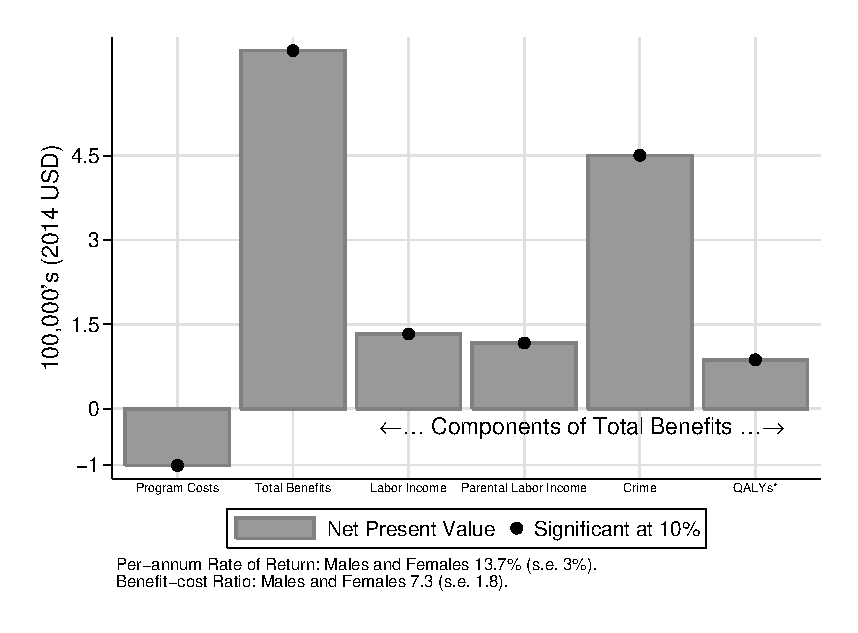
\includegraphics[width=.7\columnwidth]{output/abccare_npvssummredux.eps}
\floatfoot{
\scriptsize
Note: This figure displays the life-cycle net present values per program participant of the main components of the cost/benefit analysis of ABC/CARE from birth to forecasted death, discounted to birth at a rate of 3\%. By ``net" we mean that each component represents the total value for the treatment group minus the total value for the control group. Program costs: the total cost of ABC/CARE, including the welfare cost of taxes to finance it. Total benefits: the benefits for \textit{all} of the components we consider. Labor income: total individual labor income from age 21 to the retirement of program participants (assumed to be at age 67). Parental labor income: total parental labor income of the parents of the participants from when the participants were ages 1.5 to 21. Crime: the total cost of crime (judicial and victimization costs). To simplify the display, the following components are not shown in the figure: (i) cost of alternative preschool paid by the control-group children's parents; (ii) the social welfare costs of transfer income from the government; (iii) disability benefits and social security claims; (iv) costs of increased individual and maternal education (including special education and grade retention); (v) total medical public and private costs. Inference is based on non-parametric, one-sided $p$-values from the empirical bootstrap distribution. We indicate point estimates significant at the $10\%$ level.\\
*QALYs refers to the quality-adjusted life years. Any gain corresponds to better health conditions until forecasted death, with $\$150,000$ (2014 USD) as the base value for a year of life.\\}
\end{sidewaysfigure}


We contribute to the literature on the effectiveness of early childhood programs by considering their long-term benefits on health. We estimate the savings from life-cycle medical costs and from improvements in the quality of life.\footnote{\cite{Campbell_Conti_etal_2014_EarlyChildhoodInvestments} show the substantial adult (mid 30s) health benefits of ABC but do not present a cost/benefit analysis of their results.} There are benefits for participants in terms of reduced participation in crime, increased life-cycle labor income, reduced special education costs and enhanced educational attainment. The program subsidizes maternal childcare, thereby facilitating maternal employment, labor income, and educational attainment.

Figure~\ref{figure:main} previews our findings. It displays the discounted (using a 3\% discount rate) life-cycle benefits and costs of the program (2014 USD) pooled across genders, over all categories, and for separate categories as well.\footnote{The baseline discount rate of 3\% is an arbitrary decision. In Table~\ref{table:bcsens} and Table~\ref{table:cba}, we report benefit/cost ratios using other discount rates. Using discount rates of 0\%, 3\%, and 7\%, the estimates for the benefit/cost ratios are 17.40 (s.e. 5.90), 7.33 (s.e. 1.84), and 2.91 (s.e. 0.59), respectively. We report estimates for discount rates between 0\% and 15\% in  Appendix~\ref{appendix:varying-discount-rate}.} We report separate estimates by gender later in this paper and find substantial differences in gender effects. The costs of the program are substantial, as has frequently been noted by critics.\footnote{See, e.g., \citet{Fox_News_2014_Head_Start_Effects} and \citet{Whitehurst_2014_Senate_Testimony}.} But so are the benefits, which far outweigh the costs.

\begin{figure}[!htbp]
\caption{Benefit/Cost Ratio and Internal Rate of Return when Accounting for Different Combinations of the Main Benefits}\label{figure:vennpooled}
\centering
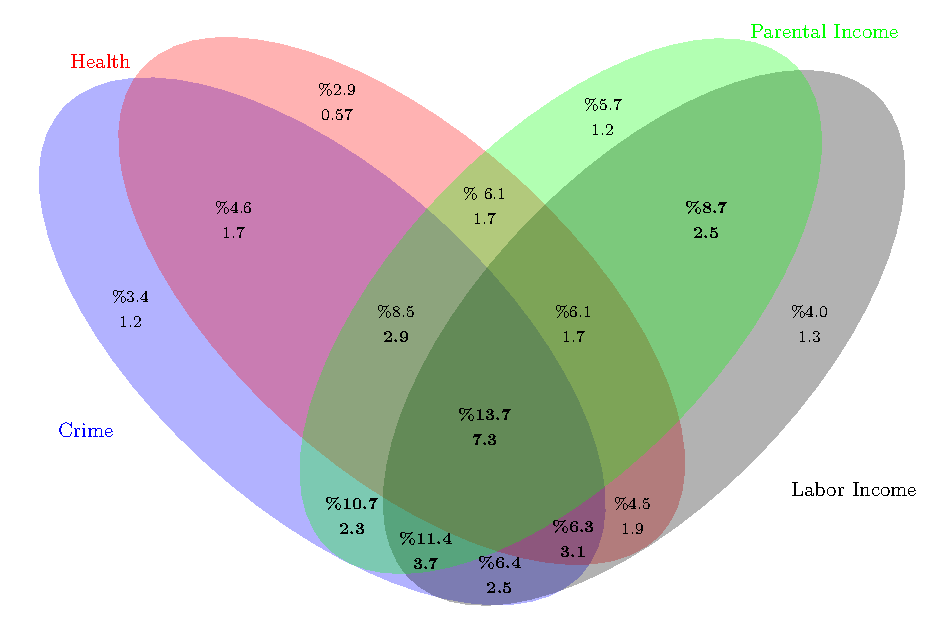
\includegraphics[width=.7\columnwidth]{output/venn_pooled.pdf}
\floatfoot{
\footnotesize
Note: This figure presents all possible combinations of accounting for the benefits from the four major categories in our analysis. The non-overlapping areas present estimates accounting for a single category as the benefit. Where multiple categories overlap, we account for benefits from each of the overlapping categories. The other components remain constant across all calculations and are the same as in Figure~\ref{figure:main}. Health combines QALYs (quality-adjusted life years) and health expenditure. Inference is based on non-parametric, one-sided $p$-values from the empirical bootstrap distribution. We put boxes around point estimates that are statistically significant at the $10\%$ level.  \\}
\end{figure}

Figure~\ref{figure:vennpooled} summarizes the results from our extensive sensitivity analyses. It shows the estimated rates of return and benefit/cost ratios when we calculate our estimates under the assumption that only one of the many streams we consider is the source of the benefit. We calculate the estimates with all possible combinations of the main benefit and cost streams. Our measures of economic efficiency remain statistically and economically significant even after eliminating the benefits from any one of the four main components that we monetize. No single component drives our results. We report estimates from a variety of specifications of regressors and functional forms. Our estimates are robust to different plausible assumptions about the values of non-market outcomes, for which conventional estimates of standard errors are not available.

Figure~\ref{figure:ranges} summarizes the range of all of the estimates that we generate in this paper. The overall benefit/cost ratio (internal rate of return) ranges from 1.52 to 17.40 (8 to 18.3) for the full sample. They range from 2.23 to 25.45 (6 to 19.4) for the males, and from 1.12 to 5.79 (4 to 18) for the females. Benefits from reductions in criminality and increased labor income are pronounced for males, contributing to their larger estimates relative to the females estimates. However, when we omit crime from our analysis, we still estimate substantial returns for males. The returns of the program are higher for males relative to attending a low-quality preschool; the returns are higher for females relative to those who stay at home.

This paper justifies and interprets these estimates. The paper unfolds in the following way. Section~\ref{section:background} discusses the ABC/CARE program. Section~\ref{section:cbamethodology} presents our notation and the definitions of the treatment effects reported in \cite{Garcia_Heckman_Ziff_2017_Gender-Diff_UNPUBLISHED} that are the basis for the estimates reported in this paper. They show that the program had substantial impacts on multiple domains. This paper reports treatment effects in economically meaningful metrics.  Section~\ref{section:cbamethodology} presents our methods for forecasting life-cycle outcomes and the evidence supporting the assumptions that justify them. Section~\ref{section:monetizing-benefits-costs} discusses how we monetize life-cycle outcomes. Section~\ref{section:cbaresults} reports our estimates of benefit/cost ratios and rates of return and the outcomes from a variety of robustness checks. Section~\ref{section:bcaestimates} examines the predictive validity of \emph{ad hoc} forecast methods currently used in the literature to estimate the long-run benefits of programs with short-term follow up. Section~\ref{section:conclusion} summarizes the paper.

\begin{sidewaysfigure}[H]
\centering
\caption{Distribution of Benefit/Cost and Internal Rate of Return Estimates}\label{figure:ranges}
\begin{subfigure}[h]{0.49\textwidth}
	\centering
	\caption{Benefit/Cost Ratio} \label{fig:bc}
	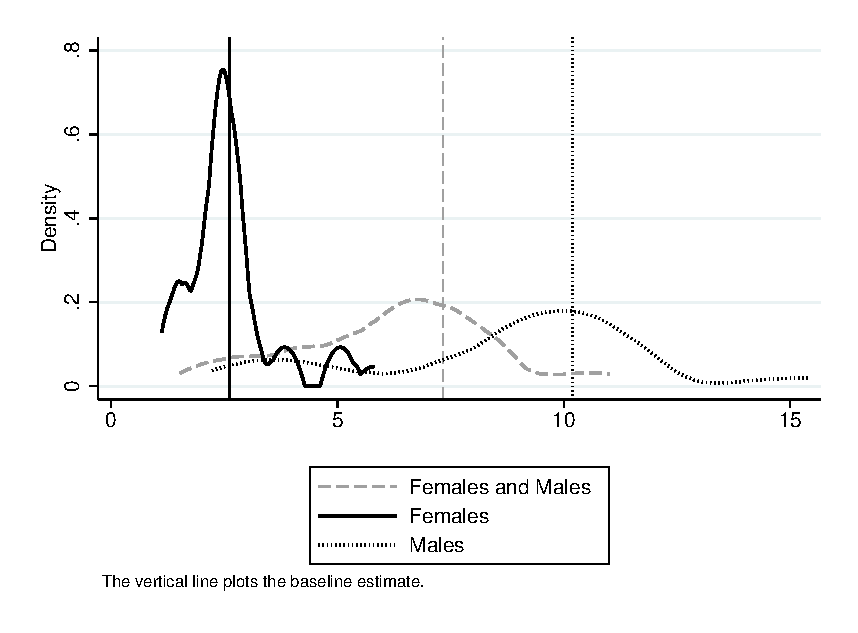
\includegraphics[width=\textwidth]{output/overalldist_BCRatio}
\end{subfigure}
\begin{subfigure}[h]{0.49\textwidth}
	\centering
	\caption{Internal Rate of Return} \label{fig:irr}
	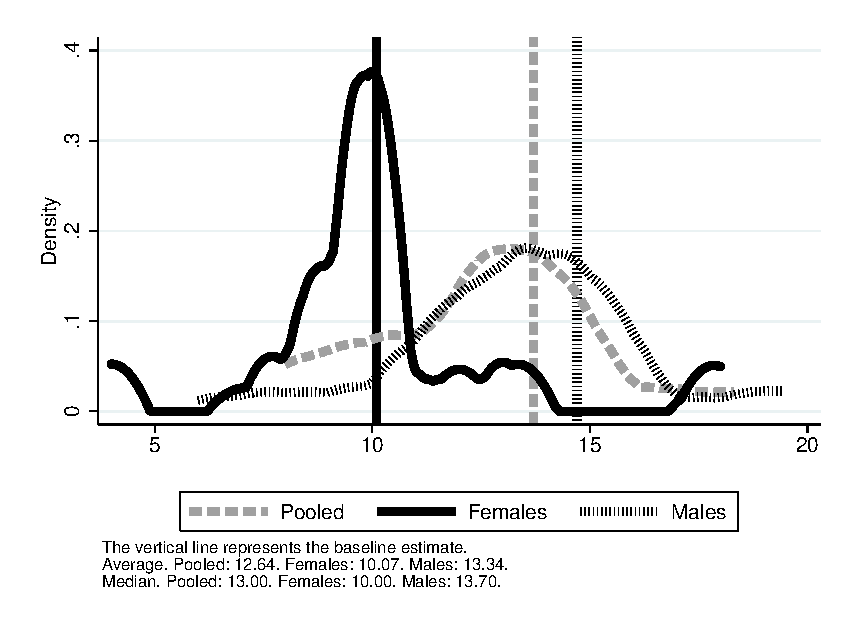
\includegraphics[width=\textwidth]{output/overalldist_IRR}
\end{subfigure}%
\footnotesize \justify
Note: Panel (a) displays the distribution of estimates of the benefit/cost ratio that we estimate throughout the paper. Vertical lines indicate the baseline estimates, presented in Figure~\ref{figure:main}. Panel (b) presents the analogous figure for the internal rate of return. See Figure~\ref{figure:ranges-NPV} in Appendix~\ref{appendix:sensitivity} for the analogous plots of net present values. \\
\end{sidewaysfigure}

\section[Background and Data Sources]{Background and Data Sources} \label{section:background}

ABC/CARE targeted disadvantaged, predominately African-American children in Chapel Hill/Durham, North Carolina.\footnote{Both ABC and CARE were designed and implemented by researchers at the Frank Porter Graham Center of the University of North Carolina in Chapel Hill.} \cite{Garcia_Heckman_Ziff_2017_Gender-Diff_UNPUBLISHED} and  Appendix~\ref{appendix:background} describe these programs in detail. Here, we summarize their main features.

The goal of these programs is to enhance the life skills of disadvantaged children. Both programs support language, motor, and cognitive development as well as socio-emotional competencies considered crucial for school success including task orientation, the ability to communicate, independence, and pro-social behavior.\footnote{\citet{Sparling_1974_Synth_Edu_Infant_SPEECH, Ramey_Collier_etal_1976_CarolinaAbecedarianProject, Ramey_etal_1985_Project-CARE_TiECSE, Wasik_Ramey_etal_1990_CD, Ramey-etal_2012-ABC}.} The programs provide health screenings to treatment group members, but health care costs are paid by parents.

ABC recruited four cohorts of children born between 1972 and 1976. CARE recruited two cohorts of children, born between 1978 and 1980. For both programs, families of potential participants were referred to researchers by local social service agencies and hospitals at the beginning of the mother's last trimester of pregnancy. Eligibility was determined by a score on a childhood risk index.\footnote{See  Appendix~\ref{app:eligibility-pop} for details on the construction of the index. It weights the following variables (listed from the most to the least important according to the index): maternal and paternal education, family income, father's presence at home, lack of maternal relatives in the area, siblings behind appropriate grade in school, family on welfare, father in unstable job, low maternal IQ, low siblings' IQ, social agency indicates that the family is disadvantaged, one or more family members has sought a form of professional help in the last three years, and any other special circumstance detected by program's staff.}

The design and implementation of ABC and CARE are very similar. Both have two phases, the first of which lasts from birth until age 5. In this phase, children are randomly assigned to treatment. The second phase of the study consists of child academic support through home visits from ages 5 through 8. The first phase of CARE, from birth until age 5, has an additional treatment arm of home visits designed to improve home environments.\footnote{\citet{Wasik_Ramey_etal_1990_CD}.} Our analysis uses the first phase and pools the CARE treatment group with the ABC treatment group. We do not use data from the CARE group that only receive home visits in the early years. \cite{Campbell_Conti_etal_2014_EarlyChildhoodInvestments} test and do not reject the hypothesis that the data sets used in this paper have a common structure.

For both programs, from birth until age 8, data were collected annually on cognitive and socio-emotional skills, home environments, family structure, and family economic characteristics. After age 8, data on cognitive and socio-emotional skills, education, and family economic characteristics were collected at ages 12, 15, 21, and 30.\footnote{At age 30, measures of cognitive skills are unavailable for both ABC and CARE.} In addition, we have access to administrative criminal records and a physician-administered medical survey when the subjects were in their mid 30s.\footnote{See  Appendix~\ref{appendix:data} for a more comprehensive description of the data. There, we document the balance in observed baseline characteristics across the treatment and control groups after dropping the individuals for whom we have no crime or health information. There is substantial attrition for these data collections. Further, the methodology we propose addresses missing data in either of these two outcome categories.}

Randomization for ABC/CARE was conducted on child pairs matched on family characteristics. Siblings and twins were jointly randomized into either treatment or control groups.\footnote{For siblings, this occurred when two siblings were close enough in age such that both of them were eligible for the program.} Randomization pairing was based on the childhood risk index, maternal education, maternal age, and gender of the subject.\footnote{We do not know the original pairs.} Dropouts are evenly balanced and are predominately related to the health of the child and mobility of families rather than dissatisfaction with the program.\footnote{The 22 dropouts in ABC include four children who died, four children who left the study because their parents moved, and two children who were diagnosed as developmentally delayed. See Table~\ref{table:abccompromises} for details. All eligible families agreed to participate. Dropping out occurs \emph{after} randomization.}

Seventy-five percent of the ABC control group and \treatsubscarec\ of the CARE control (but no children from the families offered treatment) attended alternative (to home) childcare.\footnote{See \cite{Heckman_Hohmann_etal_2000_QJE} on the issue of substitution bias in social experiments.} Those who enrolled generally stayed enrolled. As control children age, they are more likely to enter alternative childcare (see  Appendix~\ref{app:control-subbb}). Children in the control group who are enrolled in alternative early childcare programs are less economically disadvantaged at baseline compared to children who stay at home. On average, they are children with mothers who were more likely to be working at baseline.\footnote{The difference is statistically significant at 10\%.} Parents of control-group girls were much more likely than parents of control-group boys to use alternative childcare if assigned to the control group.\footnote{Most of the alternative childcare centers received federal subsidies and were subject to the federal regulations of the era ( Appendix~\ref{appendix:tetanus}). See \citet{Department-of-Health_1968_DayCareRequirements,NCGA_1971_House-Bill-100,Ramey-et-al_1977_Intro-to-ABC,Ramey_Campbell_1979_SR,Ramey_McGinness_etal_1982_Abecedarianapproach, Burchinal_Campbell_etal_1997_CD}. They had relatively low quality compared to ABC/CARE.}

\section{Forecasting Life-cycle Costs and Benefits}\label{section:cbamethodology}

This section discusses the model and data sources used to forecast life cycle profiles.

\subsection{Parameters Underlying Our Analysis}
\label{section:methodsquestions}

We begin by summarizing the treatment parameters underlying our analysis.\footnote{See \citet{Garcia_Heckman_Ziff_2017_Gender-Diff_UNPUBLISHED} for a full discussion of these parameters and the presentation of their estimates.} Toward this end, we define three indicator variables: $W = 1$ indicates that the parents referred to the program participate in the randomization protocol, $W = 0$ indicates otherwise. $R$ indicates randomization into the treatment group ($R = 1$) or to the control group ($R = 0$). $D$ indicates attending the program, i.e., $D = R$ implies compliance with the initial randomization protocol.

Individuals are eligible to participate in the program if baseline background variables $\bm{B}\in\mathcal{B}_0$. $\mathcal{B}_0$ is the set of scores on the risk index that determines program eligibility. Because all of the eligible persons given the option to participate choose to do so $(W=1\text{, and } D=R)$, we can safely interpret the treatment effects generated by the experiment as average treatment effects for the population for which $\bm{B}\in\mathcal{B}_0$ and not just treatment effects for the treated (\textbf{TOT}).\footnote{All providers of health care and social services (referral agencies) in the area of the ABC/CARE study were informed of the programs. They referred mothers whom they considered disadvantaged. Eligibility was corroborated before randomization. Our conversations with the program staff indicate that the encouragement from the referral agencies was such that most referred mothers attended and agreed to participate in the initial randomization \citep{Ramey-etal_2012-ABC}.}

Denote potential outcome $j$, $j \in \mathcal{J}_a$ at age $a \in [1, \ldots, A]$ under treatment status $d \in \{0, 1\}$ (treatment or control) in the sample $k \in \{e, n \}$, by $Y_{k,j,a}^d$. The set $\mathcal{J}_a$ indexes the outcomes of interest measured at age $a \in [1, \ldots, A]$.

All treatment group children have the same exposure. Although it would be ideal to analyze control children by the length of their exposure to alternative environments, data limitations lead us to simplify the analysis of the control substitution by creating two categories. ``$H$'' indicates that the control child is in home care throughout the entire length of the program. ``$C$'' indicates that the control child is in alternative childcare for any amount of time.\footnote{This assumption is consistent with the finding in \cite{Garcia_Heckman_Ziff_2017_Gender-Diff_UNPUBLISHED} that once parents decide to enroll their children in alternative childcare arrangements, the children stay enrolled up to age 5. They also find little sensitivity of the estimates of treatment effects to the choice of different, related categorizations.}  This separation of the counterfactual setting allows us to calculate the returns of ABC/CARE in comparison to (i) staying at home ($H$), (ii) alternative childcare ($C$), or (iii) the ``next best'' option, which pools across the full control group.

\subsection{Using Auxiliary Data Sources to Forecast Out-of-Sample Outcomes}\label{sec:usingaux}

The goal of this paper is to quantify the multiple benefits of ABC/CARE in terms of benefit/cost ratios and rates of return. We rely on auxiliary data to forecast the costs and benefits of the program over the life cycle after the measurement phase of the study ends.\footnote{See Appendix~\ref{app:datasets} for an overview of the auxiliary datasets that we use.}

\begin{sidewaystable}[!htbp]
\begin{threeparttable}
\caption{Summary of Forecast Methodology to Construct Life-cycle Costs and Benefits} \label{table:sources}
\tiny
\begin{tabular}{llllll} \toprule
    \textbf{Component} & \textbf{Subject's Age} & \textbf{Baseline Prediction Method} & \textbf{Variables Used to Construct}     & \textbf{Variables Used to Predict} & \textbf{Auxiliary Samples} \\
                    &   \textbf{at Prediction} &                                              & \textbf{Synthetic Experimental Groups}  &                                          & \textbf{Used}                         \\ \midrule
Program Costs             & 0 to 5      & Observed (source documents)      & N/A & N/A & N/A \\ \midrule
Costs of Alternative Preschools & 0 to 5      & Estimated from  & N/A & N/A & N/A \\
                           &                & Location \& Time & & & \\
                                    &                & Relevant Documents & & & \\ \midrule
Education Costs                       & up to 30  & Level is Observed                        & N/A & N/A & N/A \\
(includes special education     &                & (Per Level Cost taken             &       &        &        \\
and grade retention)                & & from NCES) & & & \\ \midrule

Labor Income       & 21 to 30 & Based on Prediction Model     & Birth-year; Gender;   & Gender; Mother's Education; & CNLSY \\
or                          &               & in the Auxiliary Sample            & Siblings at Birth     & at Birth; PIAT Math (5 to 7);   &              \\
Transfer Income   &               &                                                  &                             & Education (30)                       &              \\
                       &               &                                                  &                                   & Labor Income (21)                 &              \\
                       &               &                                                  &                                   & Lagged Outcome            &              \\ \midrule

Labor Income     & 30 to 67 & Based on Prediction Model      & Birth-year; Gender;    & Gender; Education (30);        & Pooled NLSY79  \\
or                        &               & in the Auxiliary Sample             & Siblings at Birth          & Labor Income (30);                & and PSID  \\
Transfer Income &               &                                                  &                                    & Lagged Outcome            &                   \\  \midrule

Parental Labor & 0 to 21  & Linear Interpolation       &   N/A & N/A & N/A  \\
     Income       &               & (Observed Values at     &   &       &   \\
                        &               & Ages 1.5, 2.5, 3.5, 8,    &   &       &    \\
                        &               & 12, 15, 21)                     &    &      &    \\  \midrule

Crime              & up to Mid 30s &  Observed$^*$                   &   N/A & N/A & N/A   \\
(Arrests and    &                       & (Combines Administrative & & & \\
 Sentences)    &                        &   and Self-reported Data)  & & & \\ \midrule

Crime              & Mid 30s to 50  & Based on Prediction Model      & Use Full Auxiliary     & Lagged Crime Outcomes & NCDPS \\
(Arrests and    &                       & in the Auxiliary Sample             & Sample  to Predict   &   (all outcomes listed in Table~\ref{tab:crime_cat}) & \\
 Sentences)    &                        & (One Prediction per Arrest       & Control and Treat- & & \\
                       &                        & or Sentence)                            & ment Outcomes& & \\  \midrule

Victimization   & up to Age 50  &  Impute national          & Use Full Auxiliary & N/A & NCVS; NJRP; UCRS \\
Inflation          &                        &  victims-arrests ratio   & Samples to Impute              &        & (vary by crime)   \\ \midrule

Health Costs  & before Age 30 & Based on Prediction Model & Use Full Auxiliary          & Age-specific (four follow-ups  & MEPS \\
                        &                       & in the Auxiliary Sample        & Sample  to Predict        & available) detailed                 & \\
                        &                       &                                             &                                       & in Table~\ref{table:pre30}            & \\  \midrule

Health Transitions   & 30 to Death & Based on Prediction Model & Use Full Auxiliary    & Gender; Education (30);     & PSID and        \\
(includes disability   &                   & in the Auxiliary Sample         & Samples to Predict & Lagged Health Outcomes   & HRS (only for \\
claims)                     &                   &                                               &                                & as indicated in Table~\ref{table:transition}  & mortality) \\ \midrule

Health Costs         & 30 to Death       & Based on Prediction Model & Use Full Auxiliary    & Age; Gender; Race;        & MEPS        \\
                              &                           & in the Auxiliary Sample       & Samples to Predict & Education (30); Marital    & MCBS (if Medicaid \\
                              &                           &                                             &                                & Status (30); Disease       & eligible)        \\
                              &                           &                                             &                                & Conditions; Labor Income (30) \\ \midrule
QALYs                  & 30 to Death       & Based on Prediction Model & Use Full Auxiliary    & ADL and IADL counts; & PSID  \\
                              &                          & in the Auxiliary Sample        & Samples to Predict & Disease Conditions & and MEPS \\ \midrule
Deadweight-loss   & 0 to Death         &  .50 cents per each  &   N/A        & N/A & N/A  \\
                             &                           & government-spent dollar      & & & \\  \bottomrule
                       \end{tabular}



\begin{tablenotes}
\scriptsize
Note: This table summarizes our methodology for forecasting the costs and benefits of each component that we consider. Abbreviations: ADL: Activities for Daily Living; IADL: Instrumental Activities for Daily Living; CNLSY: Children of the National Longitudinal Survey of the Youth 1979;  HRS: Health and Retirement Study; NCES: National Center of Education Statistics; NCDPS: North Carolina Department of Public Safety Data; NLSY79: National Longitudinal Survey of the Youth 1979; MEPS: Medical Expenditure Panel Survey; MCBS: Medicare Current Beneficiary Survey; NJRP: National Judicial Reporting Program; NVS: National Crime Victimization Survey; PSID: Panel Study of Income Dynamics; UCRS: Uniform Crime Reporting Statistics. N/A: not applicable. A quality-adjusted life year (QALY) reweighs a year of life according to its quality given the burden of disease. Suppose we assign a value of $\$150,000$ (2014 USD) to each year of life. A QALY of $\$150,000$ denotes a year of life in the absence of disease (perfect health). The value of QALY for an individual in a given year is smaller than $\$150,000$ when there is positive burden of disease, as worse health conditions imply a lower quality of life. When an individual dies, her QALY equals zero. There are extreme combinations of disease and disability that may generate negative QALYs, although this is unusual. Because we quantify labor income in addition to other components, this value corresponds solely to monetizing the value of life net of what individuals produce in terms of economic output. The benefit/cost ratio and internal rate of return remain significant after removing this component entirely (see Table~\ref{table:cba}). \\
$^*$When not observed, we impute based on the national arrest-sentence ratio  from NJRP and UCRS. We assume that a lack of criminal records before the mid 30s implies no crime after the mid 30s. \\
\end{tablenotes}
\end{threeparttable}
\end{sidewaystable}

This section explains our strategy for constructing out-of-sample treatment effects.\footnote{ Appendix~\ref{appendix:gmm} gives details of our step-by-step procedure and states its identification and estimation strategy in the Generalized Method of Moments framework.} Our approach builds on the analysis of \citet{Heckman_Pinto_etal_2013_PerryFactor}, who show that, for the Perry Preschool program, the effect of treatment on outcomes operates through its effects on measured inputs in a stable production function rather than through shifts in the production function. If this is also true for ABC/CARE, this feature greatly facilitates our projection analysis. We test and do not reject the hypothesis that treatment works by shifting inputs and not the production function using the ABC/CARE data.

Table~\ref{table:sources} presents the outcomes for which we conduct these analyses. It also summarizes the methodology and auxiliary samples used to make our predictions. We focus on labor income to illustrate our approach, but a similar methodology is used to forecast other outcomes.\footnote{We do not monetize the loss of leisure and household production that individuals experience from working (this applies both to the individuals in the program and to their parents). The reasons for this are two-fold: (i) we lack information on intensive-margin labor supply; and (ii) different labor supply models and market structures have different implications with respect to the value of non-market time. In addition, our data are not well-suited for estimating a structural model of labor supply. We note, however, that the benefit/cost ratio and internal rate of return are both statistically significant and substantial after removing any benefits from labor income entirely (see Table~\ref{table:cba}). This exercise corresponds to a one-to-one loss of leisure given the gain in labor income, i.e. for each additional dollar an individual makes, she loses the same dollar of (monetized) leisure and household production.}$^,$\footnote{Our calculations are based on labor income gross of tax, because we want to quantify the effects of the program on the gross output that an individual is able to produce. A rise in gross labor income increases the taxable base and has an implied increase in deadweight loss. We do not quantify that deadweight loss because: (i) we do not have enough information to make full use of standard tax simulators; and (ii) we are not able to vary the standard tax simulators to assess estimation uncertainty.} We first present an intuitive summary of our approach. We formalize these intuitions in the next section, and in the Appendix. The remaining sections apply the methodology to other outcomes besides labor income.

We have data on control- and treatment-group members through age $a^{\ast}$. We can identify treatment effects within the experimental sample at these ages. We cannot identify these treatment effects at ages for which we lack information on participant outcomes. Instead, we forecast post-$a^{\ast}$ treatment effects, which are required to construct counterfactual life-cycle profiles.

Making valid forecasts of out-of-sample treatment effects does not require making valid forecasts of separate out-of-sample treatment and control profiles. Only valid forecasts of their difference are required. We compare the predictive power of constructed treatment and control groups through age $a^*$. We also analyze the performance of forecasts of separate treatment and control profiles after age $a^*$. Doing so allows us to test the validity of our methodology by comparing (within the support of the experimental sample) outcomes by treatment status for the experimental control and treatment groups with those from the synthetic control and treatment groups we generate. Comparisons between the experimental control group and the synthetic control group are particularly compelling because neither group receives treatment.\footnote{Although some might be attending other centers. We control for participation in Head Start in our auxiliary samples. Doing so does not substantially alter our estimates. The raw difference in the net present values between treatment and control labor income is 81,230 (123,210) for females (males). This is compared to 55,720 (153,140) for the baseline estimates. We underestimate the treatment effect by not conditioning on Head Start.} Because all persons in the experimental sample who are offered treatment accept it, it is straightforward to construct synthetic control groups in auxiliary samples using only eligibility criteria.

There are two distinct stages in our analysis. In Stage I, we construct samples of individuals in the auxiliary samples with characteristics similar to those of the individuals in the experimental sample. The minimal set of characteristics includes the background variables $\bm{B} \in \mathcal{B}_0$. We use a coarse form of matching based on Algorithm~\ref{alg:match} in  Appendix~\ref{appendix:match}. In Stage II, we build models using these samples to forecast out-of-sample outcomes separately for the treated and the controls.

Stage II is implemented by a three-step procedure. In Step 1, we use the experimental sample to conduct mediation analyses relating the vector of outcomes at age $a$ for person $i$ ($\bm{Y}^{d}_{i,a}$) for $a\leq a^*$ to predictor variables (and interactions) that are affected by treatment ($\bm{X}^{d}_{i,a}$), as well as background variables ($\bm{B}_i$). It turns out that we accurately predict within-sample treatment effects as well as the levels of treatment- and control-group profiles using this approach. In Step 2, we construct counterpart forecasts of treatment and control outcomes using the auxiliary samples. We compare the constructed counterparts to the actual samples for ages $a \leq a^\ast$. In Step 3, we use the estimated dynamic relationships fit on the constructed samples to forecast the post-$a^{\ast}$ outcomes.

Under exogeneity of the predictor variables and structural invariance, the two stages can be compressed into a single, one-stage, non-parametric matching procedure.\footnote{See \citet{Heckman_Ichimura_etal_1998_Econometrica} for an example.} In  Appendix~\ref{appendix:nonpar} we compare the estimates from matching with those from our main approach and find close agreement between the two approaches and for different assumptions about the serial correlation processes of the outcome equations.

Figure~\ref{fig:labor-income-profiles} previews the results of applying the two-stage approach, displaying the life-cycle labor income profiles for the treatment and control groups. It also compares the realized labor income with the model-predicted labor income at $a^*$. There is close agreement of the constructed profiles within the age group of the experimental sample. The pattern of life-cycle labor income we generate is typical for that of low-skilled workers \citep{Blundell-etal_2015_J-Pub-E,Gladden_Taber_2000_WageProgression,Sanders-Taber_2012_AR,Lagakos_Moll_etal_2016_LifeCycle_NBER}.\footnote{For details on the variables used to construct the forecasts, see  Appendix~\ref{appendix:methodology}.}

\begin{sidewaysfigure}[!htbp]
\centering
\caption{Forecasted Labor Income Profiles for ABC/CARE Participants}\label{fig:labor-income-profiles}
\begin{subfigure}[h]{0.5\textwidth}
		\centering
		\caption{Males} \label{fig:labor-income-profilesc}
		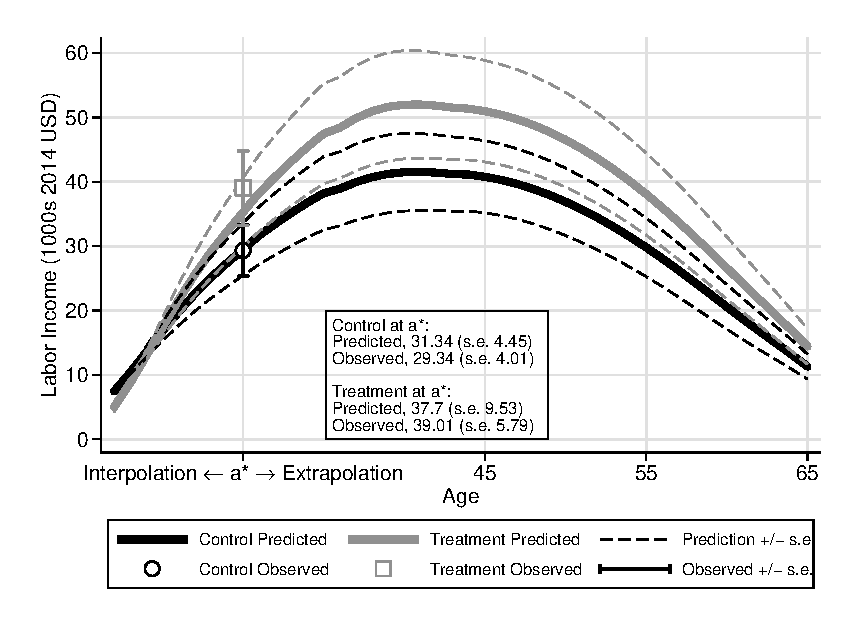
\includegraphics[width=\textwidth]{output/labor_25-65_pset1_mset1_male.eps}
\end{subfigure}%
\begin{subfigure}[h]{0.5\textwidth}
		\centering
		\caption{Females} \label{fig:labor-income-profilesa}
		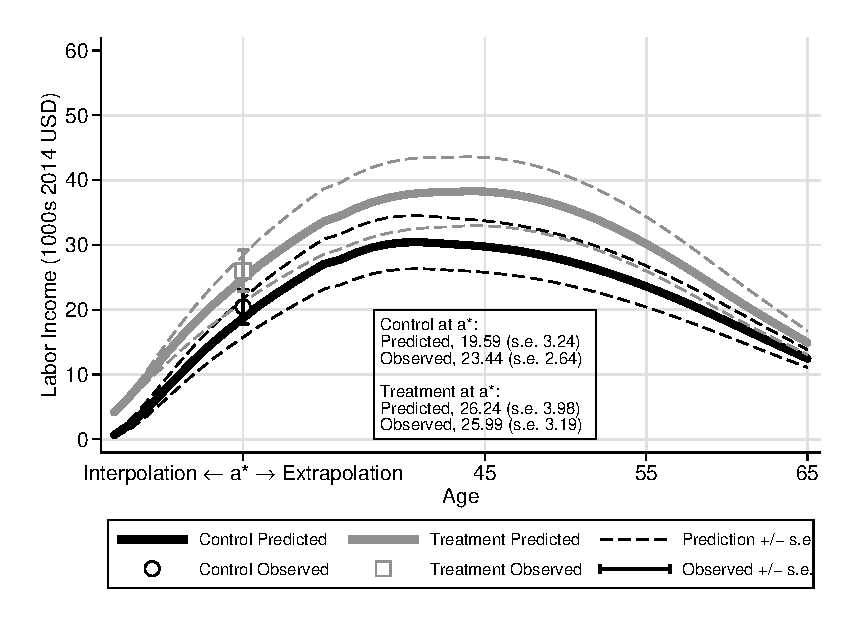
\includegraphics[width=\textwidth]{output/labor_25-65_pset1_mset1_female.eps}
\end{subfigure}
\footnotesize \justify
Note: Panel (a) displays the forecasted life-cycle labor income profiles for ABC/CARE males by treatment status, based on the method proposed in Section~\ref{sec:usingaux}. We combine data from the Panel Study of Income Dynamics (PSID), the National Longitudinal Survey of Youth 1979 (NLSY79), and the Children of the National Longitudinal Survey of Youth 1979 (CNLSY79). We highlight the \textit{observed} labor income at $a^*$ (age 30) for the ABC/CARE control- and treatment-group participants. Panel (b) displays the analogous figure for females. Our forecasts go up to age 67, the age of assumed retirement. Standard errors are based on the empirical bootstrap distribution. See Condition~\ref{cond:cond3} for a discussion of testing the difference in the observed and forecasted treatment effects (as opposed to the difference in the observed and forecasted levels). See  Appendix~\ref{appendix:methodology} for a discussion of our choice of predictors and a sensitivity analysis on those predictors. We under-predict labor income for both males and females. These differences, however, are not statistically significant (and labor income is a relatively minor component of the overall analysis for females).
\end{sidewaysfigure}

We conduct a further check on the validity of our procedure. In the experimental sample all of the parents of children with characteristics $\bm{B} \in \mathcal{B}_0$ agree to participate in the program.  Because the auxiliary samples have no treatment group members, we can evaluate our procedure by comparing the labor incomes of individuals in the auxiliary samples for whom $\bm{B} \in \mathcal{B}_0$ to the labor incomes of individuals in our constructed synthetic control group. Figure~\ref{figure:controltests} makes this comparison. It plots the average labor incomes of individuals in our auxiliary sample for whom $\bm{B} \in \mathcal{B}_0$ alongside those of the constructed synthetic control group from ages 20 to 45. It also displays the labor income of the experimental control group at $a^*$ (age 30).\footnote{The graphs stop at age 45 because we do not observe all of the components of the risk index determinants of eligibility after age 45 in the auxiliary samples. We use only a subset of this index to make life-cycle projections. These variables are effective predictors over the age range for which the full set of $\bm{B}$ is available.} The agreement is reassuringly close.

\begin{sidewaysfigure}[!htbp]
\centering
\caption{Labor Income Profile, Disadvantaged Individuals Synthetic Control Group in the Auxiliary Samples}\label{figure:controltests}
\begin{subfigure}[h]{0.5\textwidth}
		\centering
		\caption{Males}
		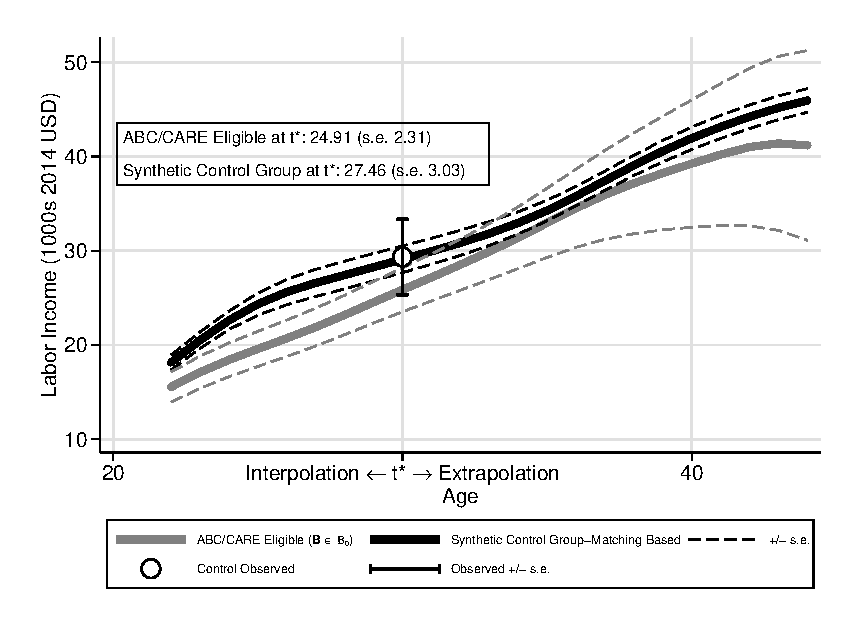
\includegraphics[width=\textwidth]{output/abccare_disad_1.eps}
\end{subfigure}%
\begin{subfigure}[h]{0.5\textwidth}
		\centering
		\caption{Females}
		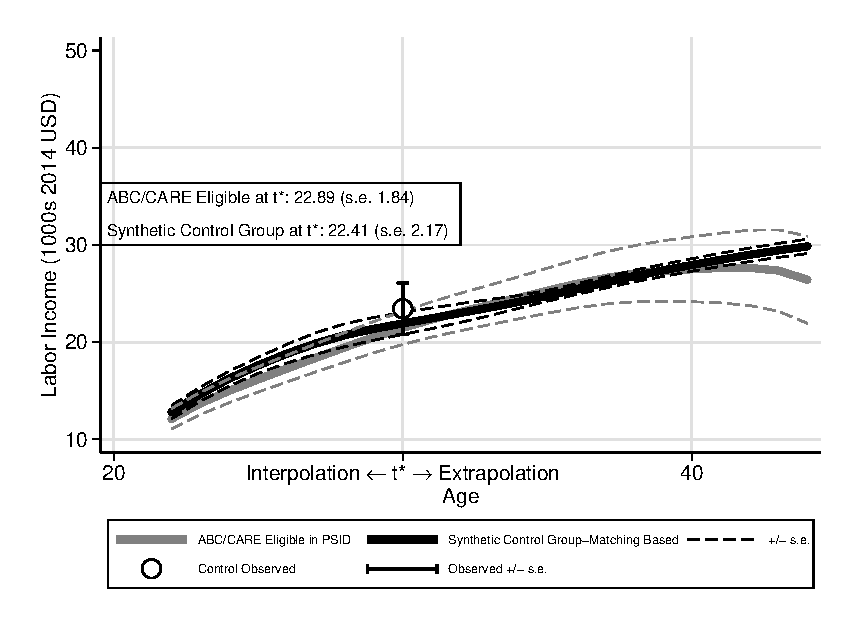
\includegraphics[width=\textwidth]{output/abccare_disad_0.eps}
\end{subfigure}
\footnotesize \justify
Note: Panel (a) displays the forecasted labor income for males in the auxiliary samples for whom $\bm{B} \in \mathcal{B}_0$, i.e., ABC/CARE eligible, and for the synthetic control group we construct based on the method proposed in this section. We combine data from the Panel Study of Income Dynamics (PSID), the National Longitudinal Survey of Youth 1979 (NLSY79), and the Children of the National Longitudinal Survey of Youth 1979 (CNLSY79). We highlight the observed labor income at $a^*$ (age 30) for the ABC/CARE control-group participants. We stop at age 45 for want of data to compute the childhood risk index defining $\bm{B} \in \mathcal{B}_0$ in the auxiliary samples. Panel (b) displays the analogous figure for females. Standard errors are based on the empirical bootstrap distribution.
\end{sidewaysfigure}

\subsection{Constructing Out-of-Sample Counterfactuals}\label{section:just}

We now formalize our analytical framework and its underlying assumptions. To avoid notational clutter, we henceforth suppress individual $i$ subscripts. Our analysis is based on a causal (structural) model for treatment ($d=1$) and control ($d=0$) counterfactual outcomes for outcome $j$ measured at age $a$ in sample $k \in \{e,n\}$, where $e$ denotes membership in the experimental sample and $n$ denotes membership in the auxiliary sample:
\begin{equation}\label{eq:outcome}
Y^d_{k,j,a} = \phi^d_{k,j,a} (\bm{X}^d_{k,a}, \bm{B}_k) + \varepsilon^d_{k,j,a}, \quad j \in \mathcal{J}_a,
\end{equation}
where $\phi^d_{k,j,a}\left( \cdot, \cdot \right)$ is an invariant structural production relationship mapping inputs $\bm{X}^d_{k,a}, \bm{B}_k$ into output $Y^d_{k,j,a}$ holding error term $\varepsilon^d_{k,j,a}$ fixed.\footnote{Fixing and conditioning are fundamentally different concepts. See \cite{Haavelmo_1943_Econometrica} and \citet{Heckman_Pinto_2015_EconometTheory} for discussions. Our analysis applies the methodology of these papers.} We normalize $\varepsilon^d_{k,j,a}$ to have mean zero. Among the $\bm{X}^d_{k,a}$ are variables caused by treatment, including lagged dependent variables. In this general framework, the relationships between the dependent and right-hand side variables in Equation~\eqref{eq:outcome} do not necessarily coincide across the samples, $k \in \{e,n\}$.

Let $\bm{Y}_k^d$ denote the vector of all outcomes at all ages for $k \in \{e, n \}$, when treatment status is fixed to $d$. Similarly, $\bm{X}_k^d$ is the vector of all causal predictors of $\bm{Y}_k^d$ at all ages. Both $\bm{Y}_k^d$ and $\bm{X}_k^d$ include the full set of possible outcomes over the life cycle, even though they are not observed after age $a^*$. The background variables may have different distributions in the two samples. We denote the joint distribution of these vectors conditional on $\bm{B}_k = \bm{b}$ by $F_{\bm{Y}_k^d, \bm{X}_k^d | \bm{B}_k = \bm{b}}(\cdot,\cdot)$.

In the experimental sample, parents of eligible children ($\bm{B}_e \in \mathcal{B}_{0}$), always agree to participate in the program ($W_e = 1$) and accept treatment ($R_e = D_e$). We assume that this condition holds in the auxiliary sample. Given this condition, we can use $D_e$ and $R_e$ interchangeably and apply a standard \citet{Quandt_1972_JASA} switching regression model to write the outputs and inputs generated by treatment as
\begin{spacing}{1}
\begin{align}\label{eq:countersystem}
Y_{k,j,a} =& \left( 1 - D_k \right) Y_{k,j,a}^0 + \left( D_k \right) Y_{k,j,a}^1, \\
&&j \in \mathcal{J}_a, a \in \{1,\dots,A\}, \quad k \in \{e,n\} \nonumber \\
\bm{X}_{k,a} =& \left( 1 - D_k \right) \bm{X}_{k,a}^0 + \left( D_k \right) \bm{X}_{k,a}^1.\nonumber\footnotemark
\end{align}
\end{spacing}
\footnotetext{We keep the conditioning on $\bm{B} \in \mathcal{B}_0$ implicit.}
\noindent The fact that $D_e = R_e$ allows us to use experimental data (for $a \in \{1, \dots,a^*\}$) to identify the distribution of $Y_{e,j,a}^d$ (i.e., $Y_{e,j,a}^d$ when fixing treatment status ($d$)).

\subsubsection{Accounting for Age, Period, and Cohort Effects}
\label{sec:accoutning-age-period-cohort}
The auxiliary data $(n)$ come from older cohorts not exposed to the program, for whom we observe more complete segments of their life cycles. We do not observe what treatment status $d$ would have been in the auxiliary data. Even if we did, we do not know if cohort ($c$) or time ($t$) effects make the experiences of the individuals in the auxiliary sample different from the experiences of the individuals in the experimental sample.

To formalize this problem, and our solution to it, let $Y_{j,k,a,c,t}^d$ be outcome $j$ for sample $k$ at age $a$ for birth cohort $c$ at time $t$ when treatment is fixed to $d$. We make the following assumption. It allows us to circumvent the problem by assuming cohort and time effects operate identically across the experimental ($e$) and non-experimental ($n$) samples in the following sense:

\onehalfspacing
\begin{assumption}\label{ass:alignment} \textbf{Alignment of Cohort and Time Effects}\\
For experimental sample cohort $c_{e}$ and auxiliary sample cohort $c_{n}$:
\begin{equation}
Y_{e,a,c_{e},t_{e}}^d = Y_{n,a,c_{n},t_{n}}^d
\end{equation}
for $d \in \{ 0, 1\}$, $a \geq a^*$, where $t_{e}, t_{n}$ are the years for which cohorts $c_{e}, c_{n}$ are observed, where $t_e = t_n + c_e - c_n$, and $t_n$ is the year that the age $a$ outcome is observed for cohort $n$ ($t_n = a + c_n$). $\square$
\end{assumption}
\doublespacing

Notice that $Y^d_{n,a,{c_n},{t_n}}$ is the outcome for treatment status $d$ in the auxiliary sample. Assumption~\ref{ass:alignment} does not rule out cohort or period effects. However, it rules out any \emph{differences} in cohort and time effects of the auxiliary sample and the experimental sample when they reach the age of those in the auxiliary sample.

We henceforth drop the ``$c$'' and ``$t$'' sub-indices. The out-of-sample year effect for the experimental sample is assumed to be the same as for the auxiliary sample measured at year $t_n$. We can weaken Assumption~\ref{ass:alignment} if there is prior knowledge about year and/or cohort effects or if we can parameterize estimable functions of $c$ and $t$.\footnote{See \cite{Heckman_Robb_1985_JE}. For health, cohort effects could be very substantial (e.g., the growth of medical costs) and we account for this as explained in Section~\ref{section:health} and  Appendix~\ref{appendix:health}.} In the sensitivity analyses reported below, we examine plausible alternative assumptions about cohort and time effects drawing on results in the empirical literature. Examples include a rate of decay in labor income due to a time effect as a crisis or a cohort effect due to skill depreciation. We also consider wage increases due to alternative scenarios of gains in productivity, or time effect due to plausible changes in the structure of medical costs.

\subsubsection{Support Conditions}

We require that the support of the auxiliary sample contains the support of the experimental sample. This assumption allows us to find counterpart values of $\bm{X}^d_{k,a}$, $\bm{B}$, and $\bm{Y}_{k,a}$ in the control and experimental samples.

\onehalfspacing
\begin{assumption} \label{ass:contain} \textbf{Support Conditions} \\
For $a \in \{ 1, \ldots, A \}$, the support of $\left( \bm{Y}^d_{e,a}, \bm{X}^d_{e,a}, \bm{B}_e \right)$ in the experimental sample is contained in the support of $\left( \bm{Y}^d_{n,a}, \bm{X}^d_{n,a}, \bm{B}_n \right)$ in the auxiliary sample:
\begin{equation}
supp( \bm{Y}_{e,a}, \bm{X}^d_{e,a}, \bm{B}_e ) \subseteq supp( \bm{Y}_{n,a}, \bm{X}^d_{n,a}, \bm{B}_n ), \quad d \in \{0,1\}. \quad \square
\end{equation}
\end{assumption}
\doublespacing
This assumption is straightforward to test for ages $a\leq a^\ast$. It is satisfied in our samples, as shown in Appendix~\ref{app:containsupport}.

\subsubsection{Conditions for Valid Out-of-Sample Forecasts}

A strong sufficient condition for identifying the distribution of life-cycle profiles of individuals in the experimental sample using individuals in the auxiliary samples is Condition~\ref{cond:cond1}:

\onehalfspacing
\begin{condition} \textbf{Equality of Distributions Across the Experimental and Auxiliary Samples \label{cond:cond1}}
\begin{equation}
F_{\bm{Y}_e^d, \bm{X}_e^d | \bm{B}_e = \bm{b}} \left( \cdot, \cdot \right) = F_{\bm{Y}_n^d, \bm{X}_n^d | \bm{B}_n = \bm{b}} \left( \cdot, \cdot \right), \quad d \in \{0,1\}
\end{equation}
\noindent for $\bm{Y}_e^d, \bm{X}^d_e | \bm{B}_e = \bm{b}$ and $\bm{Y}_n^d, \bm{X}^d_n | \bm{B}_n = \bm{b}$ contained in the support of the experimental sample $supp\left(\bm{Y}^d_{e}, \bm{X}^d_{e}, \bm{B}_{e} \right)$.
\end{condition}
\doublespacing

Since we are only interested in means for benefit/cost analysis, we can get by with a weaker requirement for conditional means, which has testable implications, as we show below:

\onehalfspacing
\begin{condition} \textbf{Equality in Conditional Expectations Across the Experimental and Auxiliary Samples \label{cond:cond2}}
\begin{equation}
\mathbb{E} \left[ \bm{Y}_e^d |  \bm{X}_e^d = \bm{x}, \bm{B}_e = \bm{b} \right] = \mathbb{E} \left[ \bm{Y}_n^d |  \bm{X}_n^d = \bm{x}, \bm{B}_n = \bm{b} \right], \quad d \in \{0,1\}
\end{equation}
for $d \in \{0, 1 \}$ over $supp\left(\bm{Y}^d_{e,a}, \bm{X}^d_{e,a}, \bm{B}_e\right)$.
\end{condition}
\doublespacing

Since we are primarily interested in treatment effects, we can get by with an even weaker condition:

\onehalfspacing
\begin{condition} \textbf{Equality in Mean Treatment Effects Across the Experimental and Auxiliary Samples \label{cond:cond3}}
\begin{equation}
\mathbb{E} \left[ \bm{Y}_e^1 - \bm{Y}_e^0 | \bm{B}_e = \bm{b} \right] = \mathbb{E} \left[ \bm{Y}_n^1 - \bm{Y}_n^0 | \bm{B}_n = \bm{b} \right]
\end{equation}
over $supp\left(\bm{Y}^d_{e,a}, \bm{B}_e\right)$.\footnotemark
\end{condition}
\footnotetext{We test the difference between the observed and forecasted treatment effect, because as we describe above, an equal difference (as opposed to equal levels) is sufficient. Even though the point estimate of the difference is 2,037.08 ($-$2,256.09) for males (females, we find that this difference is not statistically different than 0 for both genders).}
\doublespacing
We could simply invoke Condition~\ref{cond:cond2} or \ref{cond:cond3} and be done. Our approach is to examine and test (when possible) assumptions that justify the treatment effects, and Condition~\ref{cond:cond2} is useful for doing so.

\subsubsection{Exogeneity}

Conditions~\ref{cond:cond1} to \ref{cond:cond3} do not require that we take a position on the exogeneity of $\bm{X}^d_k, \: k \in \{e,n\}$. However, exogeneity facilitates the use of economic theory to generate and interpret treatment effects, to test the validity of our synthetic control groups, and to find auxiliary sample counterparts to treatments and controls. It also facilitates matching, one of the methods used in this paper to construct synthetic treatment and control groups.\footnote{See \cite{Heckman_Navarro_2004_REStat}.} For these purposes, we assume:

\onehalfspacing
\begin{assumption}\label{ass:exog} \textbf{Exogeneity}\\
For all $a, a'' \in \{ 1, \ldots, A \}$ and for $d, d' \in \{0,1\}$,
\begin{equation}
\varepsilon^d_{k,j,a} \indep \bm{X}^{d^{\prime}}_{k,a^{''}} | \bm{B}_k = \bm{b}
\end{equation}
for all $\bm{b}$ in the support of $\bm{B}_k, \: k \in \{e,n\}$, for all outcomes $j \in \mathcal{J}_{a}$, where ``$\bm{M} \indep \bm{N}|\bm{Q}$'' denotes independence of $\bm{M}$ and $\bm{N}$ given $\bm{Q}$. $\square$
\end{assumption}
\doublespacing

Assumption~\ref{ass:exog} is much stronger than needed. It justifies Conditions~\ref{cond:cond1} and~\ref{cond:cond2}, but these conditions only require that endogeneity processes are governed by the same relationships in the experimental and auxiliary samples. However, when this assumption and our other assumptions hold, we generate testable implications of our forecasting model.

To appreciate the benefit of Assumption~\ref{ass:exog}, consider the following example. Say we want to predict future labor income and we use years of education as a main component of $\bm{X}_{k,{a''}}^{d'}$. The joint distribution of $\varepsilon_{k,j,a}^d$ and $\bm{X}_{k,{a''}}^{d'}$ could differ substantially across experimental and non-experimental samples. In the experimental sample, years of education are increased by treatment, which is randomly assigned. In the non-experimental samples, however, there is no treatment. Individuals with high observed levels of education could very well have a high value of  $\varepsilon_{k,j,a}^d$ (e.g., ability bias). Assumption~\ref{ass:exog} avoids this problem when making forecasts. However, under further assumptions, it is testable and fixable.

In Appendix~\ref{app:endogeneity}, we test Assumption~\ref{ass:exog} for a variety of outcomes and fail to reject the null of exogeneity. We discuss these tests in Section~\ref{section:accendog}. In Appendix~\ref{appendix:predsensitivity}, we analyze standard panel data models for the outcome equations as well as instrumental variable approaches to account for lagged dependent variables and serial correlation. Our estimates are robust even when we allow for different failures of Assumption~\ref{ass:exog}. We also present non-parametric matching estimates. Their near-coincidence with the matching estimates with those from the structural model is further support of the validity of Assumption~\ref{ass:exog}.

\subsubsection{Structural Invariance}
\label{sec:structural-invariance}

We assume that the variables $\bm{X}_{k,a}^d$ fully summarize treatment in the sense that any effect that treatment has on outcomes operates through the inputs, $\bm{X}_{k,a}^d$, and not through shifts in the production function relating inputs to outputs (see \citealp{Heckman_Pinto_etal_2013_PerryFactor}). Assumption~\ref{ass:summary} formalizes this condition.

\onehalfspacing
\begin{assumption} \label{ass:summary} \textbf{Structural Invariance}\\
For all $\bm{x}, \bm{b} \in supp(\bm{X}^d_{e,a}, \bm{B}_e), k \in \{e,n\}$
\begin{align}
\phi_{k,j,a}^0 \left( \bm{x}, \bm{b} \right) &= \phi_{k,j,a}^1 (\bm{x}, \bm{b}) \\   \nonumber
                                                                     &=: \phi_{j,a} (\bm{x}, \bm{b}),
\end{align}
$\phi^d_{k,j,a}(\bm{x})$ is the function generating the causal effect of setting $\bm{X}^d_{k,a}=\bm{x}$ holding $\varepsilon^d_{k,j,a}$ fixed for $a \in \{1,\dots,A\}$ for any outcome $j \in \mathcal{J}_{a}$. $\square$
\end{assumption}
\doublespacing

This assumption has two distinct aspects which could be broken down into two separate assumptions: (i) the structural functions evaluated with the same arguments have identical values for treatment and control groups in the experimental sample, and (ii) the structural relationships are identical in the experimental and auxiliary samples. As previously noted, exogeneity is not needed to justify Conditions~\ref{cond:cond1} through \ref{cond:cond3}. But in the absence of exogeneity, the relationship between the inputs, $\bm{X}^d_{k,a}$, and the errors, $\bm{\varepsilon}^d_{k,a}$, likely differs across experimental ($e$) and non-experimental ($n$) samples because randomization imparts a source of exogenous variation to $\bm{X}^d_{e,a}$ that is absent in non-experimental samples.

\subsubsection{Testing Exogeneity}\label{section:accendog}

In  Appendix~\ref{app:endogeneity}, we report tests for endogeneity in the experimental and auxiliary samples used in this paper. We assume that $\varepsilon_{k,j,a}^d, , k \in \{e,n\}$ follows a factor structure.\footnote{Factor structure models are widely used in structural estimation of production functions of skills during early childhood. See, e.g., \cite{Cunha_Heckman_2008_JHR,Cunha_Heckman_etal_2010_est_tech_cognoncog} and \cite{Agostinelli_Wiswall_2016_EstimatingTech}.} We provide evidence supporting exogeneity in both samples for the predictor variables used in our empirical analyses. Once we condition on $\bm{X}_{k,a}^d$ and $\bm{B}_{k}$, we do not reject the null hypothesis of exogeneity.

\subsubsection{Testable Implications}

Assumption~\ref{ass:summary} combined with Assumption~\ref{ass:exog}, Equation~\eqref{eq:countersystem}, and the assumption $\mathbb{E}(\varepsilon^d_{k,j,a})=0$ for all $a \in \{1,\dots,A\}$ generate testable restrictions for our forecasting models. Exogeneity and invariance enable us to jointly test the two aspects of structural invariance for $a \leq a^*$, when $Y_{k,j,a}$ is observed in both the experimental and auxiliary samples:

\begin{eqnarray}
\mathbb{E} \left[ Y_{e,j,a}^1 | \bm{X}_{e,a}^1 = \bm{x}, \bm{B}_{e} = \bm{b}, D = 1   \right] &=&  \mathbb{E} \left[ Y_{e,j,a}^0 | \bm{X}_{e,a}^0 = \bm{x}, \bm{B}_{e} = \bm{b}, D = 0   \right]  \\
\text{ and} & \nonumber \\
\mathbb{E} \left[ Y_{e,j,a}^d | \bm{X}_{e,a}^d = \bm{x}, \bm{B}_{e} = \bm{b}, D = d   \right] &=&  \mathbb{E} \left[ Y_{n,j,a} | \bm{X}_{n,a} = \bm{x}, \bm{B}_{n} = \bm{b} \right] \text{ for }  d \in \{0,1\}.
\end{eqnarray}
Under our assumptions, experimental treatment effects should equal differences in the conditional means of the non-experimental samples evaluated at $\bm{X}_{n,a} = \bm{x}^1$ and  $\bm{X}_{n,a} = \bm{x}^0$:

\begin{eqnarray}
\mathbb{E} \left[ Y_{e,j,a}^1 |  \bm{X}_{e,a}^1 = \bm{x}^1, \bm{B}_e = \bm{b}, D = 1 \right] - \mathbb{E} \left[ Y_{e,j,a}^0 |  \bm{X}_{e,a}^0 = \bm{x}^0, \bm{B}_e = \bm{b}, D = 0 \right] = \nonumber \\
\mathbb{E} \left[ Y_{n,j,a} | \bm{X}_{n,a} = \bm{x}^1, \bm{B}_n = \bm{b} \right] - \mathbb{E} \left[ Y_{n,j,a} | \bm{X}_{n,a} = \bm{x}^0, \bm{B}_n = \bm{b} \right].
\end{eqnarray}
In Appendix~\ref{app:invariance}, we test and do not reject all three hypotheses, singly and jointly for $a\leq a^*$.\footnote{This holds when pooling males and females and when testing separately by gender (see  Appendix~\ref{app:invariance}).}

\subsubsection{Summarizing the Implications of Exogeneity and Structural Invariance}

Collecting results, we obtain the following theorem:

\onehalfspacing
\setcounter{theorem}{0}
\begin{theorem}\label{theorem:main} \textbf{Valid Out-of-Sample Forecasts} \\
Under Assumptions~\ref{ass:alignment}-\ref{ass:summary}, Conditions~\ref{cond:cond2} and \ref{cond:cond3} hold for any value of $\left( \bm{X}^d_{k,a}, \bm{B}_k \right)$. \\
\emph{This is an immediate consequence of the cited assumptions.} $\Box$
\end{theorem}
\doublespacing

\subsubsection{Using Matching to Construct Virtual Treatment and Comparison Groups}\label{usingmatching}

Under exogeneity assumption~\ref{ass:exog} and invariance condition~\ref{ass:summary} we can use matching to construct counterparts to the experimental treatment and control groups in the auxiliary sample.\footnote{\citet{Heckman_Ichimura_etal_1998_Econometrica} use this procedure.} Doing so compresses the two stages of constructing a comparison group and creating forecasts into one stage. Matching in this fashion creates direct counterparts in the auxiliary samples for each member of the experimental samples. It is an intuitively appealing non-parametric estimator that is valid under exogeneity \citep{Heckman_Navarro_2004_REStat}.

We discuss this approach in Appendix~\ref{appendix:match}. Matching is a non-parametric estimation procedure for conditional mean functions. There is close agreement between non-parametric estimates based on matching and more parametric model-based approaches used in most of this paper (see  Appendix~\ref{appendix:nonpar}).

\begin{sidewaystable}[H]
\resizebox{\columnwidth}{!}{%
\begin{threeparttable}
\caption{Net Present Value of Labor Income and Cost/Benefit Analysis Under Different Specifications for Labor Income Process}
\label{table:predsens}
\centering
\footnotesize
\begin{tabular}{L{2cm} *7{C{1.5cm}}} \toprule
& \multicolumn{3}{c}{ \textbf{Specification 1:}} & & \multicolumn{3}{c}{ \textbf{Specification 2:}}\\
& \multicolumn{3}{c}{Lagged component in $\bm{\phi}_{j,a}$} & & \multicolumn{3}{c}{No lagged component in $\bm{\phi}_{j,a}$} \\
& \multicolumn{3}{c}{ set $\bm{\rho} = 0$} & & \multicolumn{3}{c}{Unrestricted $\bm{\rho}$} \\[10pt]

& NPV & IRR & B/C & & NPV & IRR & B/C \\

\hline \\
Pooled & 71,345 & 0.13 & 6.29 & & 154,547 & 0.26 & 12.39 \\ 
& (86,343) & (.05) & (2.11) & & (187,036) & (0.11) & (5.16) \\ \\

Males & 300,896 & 0.13 & 11.1 & & 200,509 & 0.09 & 7.62 \\ 
& (241,588) & (0.06) & (6.35) & & (160,988) & (0.04) & (3.73) \\ \\ 

Females & 59,390 & 0.10 & 2.45 & & 79,441 & 0.15 & 3.61 \\ 
& (63,060) & (0.07) & (0.79) & & (99,416) & (0.11) & (1.56) \\ \\ \\

\midrule
& \multicolumn{3}{c}{ \textbf{Specification 3:}} & & \multicolumn{3}{c}{ \textbf{Specification 4:}}\\
& \multicolumn{3}{c}{Lagged component in $\bm{\phi}_{j,a}$} & & \multicolumn{3}{c}{Lagged component in $\bm{\phi}_{j,a}$; Permanent} \\
& \multicolumn{3}{c}{Unrestricted $\bm{\rho}$} & & \multicolumn{3}{c}{Transitory unobserved components} \\[10pt]

& NPV & IRR & B/C & & NPV & IRR & B/C \\

\hline \\
Pooled & 268,179 & 0.49 & 23.64 & & 46,953 & 0.09 & 4.14 \\ 
& (211,089) & (0.12) & (5.16) & & (25,323) & (0.01) & (0.62) \\ \\

Males &456,078 & 0.2 & 16.82 & & 74,775 & 0.03 & 2.76 \\ 
& (358,534) & (0.09) & (9.42) & & (54,752) & (0.01) & (1.44)  \\ \\ 

Females & 31,303 & 0.05 & 1.29 & & 19,959 & 0.03 & 0.82 \\ 
& (168,160) & (0.19) & (2.11) & & (34,142) & (0.04) & (0.43) \\ \\ \\


\midrule
& & & \multicolumn{3}{c}{\textbf{Specification 5:}} \\
& & & \multicolumn{3}{c}{ Fully Non-Parametric} \\[10pt]
& & & NPV & IRR & B/C \\
\hline \\
& & Pooled & 62,080 & 0.10 & 4.98 \\ 
& & & (75,030) & (0.03) & (2.07) \\ \\ 
& & Males & 289,471 & 0.13 & 11.01 \\ 
& & & (232,471) & (0.06) & (5.39) \\ \\ 
& & Females & 59,163 & 0.11 & 2.69 \\ 
& & & (74,039) & (0.08) & (1.16) \\ \bottomrule
\end{tabular}
\begin{tablenotes}
\normalsize
\item Note: This table displays the net present value of labor income in 2014 USD (treatment - control) using the five different specifications for forecasts that are explained below. Specification 1 is our baseline estimate. It also presents the calculation of the internal rate of return and the benefit/cost ratio of the program using these different net present values. Specification 1: forecast based on lagged outcome; no serial autocorrelation; and no fixed effect. Specification 2: forecast based on lagged outcome; arbitrary serial autocorrelation; and no fixed effect. Specification 3: forecast based on lagged outcome; first-order serial autocorrelation; and no fixed effects. Specification 4: forecast based on lagged outcome; no serial autocorrelation; and fixed effect. Specification 5: Forecast based on non-parametric matching estimates described in Section~\ref{usingmatching}.
\item Model: With the exception of Specification 5, the different specifications are particular cases of the following model:

\begin{large}
\begin{eqnarray}
Y_{k,j,a}                   &=& \lambda_{0} + \lambda_{1} Y_{k,j,a-1} + \lambda_{2}  \bm{X}_{k,a} + \varepsilon_{k,j,a} \nonumber \\
\varepsilon_{k,j,a} &=& \underbrace{f}_{\text{Person-Specific Effect}} + \underbrace{\omega_{k,j,a}}_{\text{Possibly Serially Correlated Component}} \nonumber \\
\omega_{k,j,a}      &=& \rho \omega_{k,j,a-1} + \underbrace{U_{k,j,a}}_{\text{Independent Innovation}}.
\end{eqnarray}
\end{large}

\end{tablenotes}
\end{threeparttable}
}
\end{sidewaystable}

\subsubsection{Exploring the Impact of Other Forecast Models} \label{section:predsensitivity}

In Appendix~\ref{appendix:predsensitivity}, we analyze the consequences of using more general forecast models that allow us to relax exogeneity Assumption~\ref{ass:exog}. We estimate standard panel data specifications. We summarize the results from these exercises for the case of forecasting labor income in Table~\ref{table:predsens} with a comprehensive note at the base of the table. Forecasts of present values exhibit little sensitivity across these different methods, and do not differ substantially from the prediction baseline model.

\section{Monetizing Specific Components of the Benefits and Costs}
\label{section:monetizing-benefits-costs}

This section discusses how we calculate the benefits and costs of health, parental income, crime, and the costs of the program. We discuss our measures of educational attainment and costs in Appendix~\ref{appendix:education}.

\subsection{Health} \label{section:health}

A major contribution of this paper is forecasting and monetizing the life-cycle benefits of enhanced participant health using a version of Equation~\eqref{eq:outcome} including a full vector of lagged dependent variables for different indicators of health status. This requires adapting the models of Section~\ref{section:just}, as well as estimating a dynamic model of competing health risks \citep{Kalbfleisch_Prentice_1980_failure}. Three additional issues arise: (i) health outcomes such as diabetes or heart disease are absorbing states; (ii) health outcomes are highly interdependent within and across time periods; and (iii) there is no obvious terminal time period for benefits and costs except death, which is endogenous.\footnote{For example, we extrapolate labor income until the retirement age of 67. However, for health, we need to forecast an age of death for each individual before extrapolating.}

Our auxiliary model for health is an adaptation of the Future America Model (FAM). This model forecasts health outcomes from the subjects' mid 30s up to their projected age of death \citep{Goldman_etal_2015_Future-Elderly-Model-Report}.\footnote{The simulation starts at the age in which we observe the subjects' age-30 follow-up.}  Appendix~\ref{appendix:health} discusses the FAM methodology in detail.

FAM passes a variety of specification tests and accurately forecasts health outcomes and healthy behaviors.\footnote{In Appendix~\ref{appendix:health-validation}, we present tests of the model's assumptions and predictive performance for population aggregate health and healthy behavior outcomes.} We initialize the health forecast model using the same variables that we use to forecast labor and transfer income, along with the initial health conditions as listed in Table~\ref{table:transition}.

Our methodology has five steps: (i) estimate age-by-age health state transition probabilities using the Panel Study of Income Dynamics (PSID); (ii) match these transition probabilities to the ABC/CARE subjects based on observed characteristics; (iii) estimate quality-adjusted life year (QALY) models using the Medical Expenditure Panel Survey (MEPS) and the PSID; (iv) estimate medical cost models using the MEPS and the Medicare Current Beneficiary Survey (MCBS), allowing estimates to differ by health state and observed characteristics; and (v) forecast the medical expenditures and QALYs that correspond to the simulated individual health trajectories.\footnote{As an intermediate step between (i) and (ii), we impute some of the variables used to initialize the FAM models (see  Appendix~\ref{section:FAM_ABC_impute}).}

Our microsimulation model starts with information on observed characteristics at age 30, along with the information on observed characteristics available at this age. Restricting it to the individuals for whom we have information from the mid 30s health survey allows us to account for components that are important for forecasting health outcomes. The models forecast the probability of being in any of the states in the horizontal axis of Table~\ref{table:transition} at age $a+1$ based on the state at age $a$, which is described by the vertical axis of the table.\footnote{In practice, the forecasts are based on two-year lags, due to data limitations in the auxiliary sources we use to simulate the FAM. For example, if the individual is 30 (31) years old in the age-30 interview, we simulate the trajectory of her health status at ages 30 (31), 32 (33), 34 (35), and so on until her projected death.} Absorbing states are an exception. For example, heart disease at age $a$ does not enter in the estimation of transitions for heart disease at age $a+1$ because it is an absorbing state: once a person has heart disease, she carries it through the rest of her life.

At each age, once we obtain the transition probability for each health outcome, we make a Monte-Carlo draw for each subject. Each simulation depends on each individual's health history and on her particular characteristics. For every simulated trajectory of health outcomes, we forecast the life-cycle medical expenditure using the models estimated from the MEPS and the MCBS. We then obtain an estimate of the expected life-cycle medical expenditure by taking the mean of each individual's simulated life-cycle medical expenditure.

The models estimated using MCBS represent medical costs in the years 2007--2010. The MEPS estimation captures costs during 2008--2010. To account for real medical cost growth after 2010, we adjust each model's forecast using the method described in  Appendix~\ref{appendix:health-fam-simulation}.

\begin{figure}[!htbp]
\caption{Mean Quality-Adjusted Life Years: Forecasts and Comparison to PSID}\label{fig:qalys}
\centering
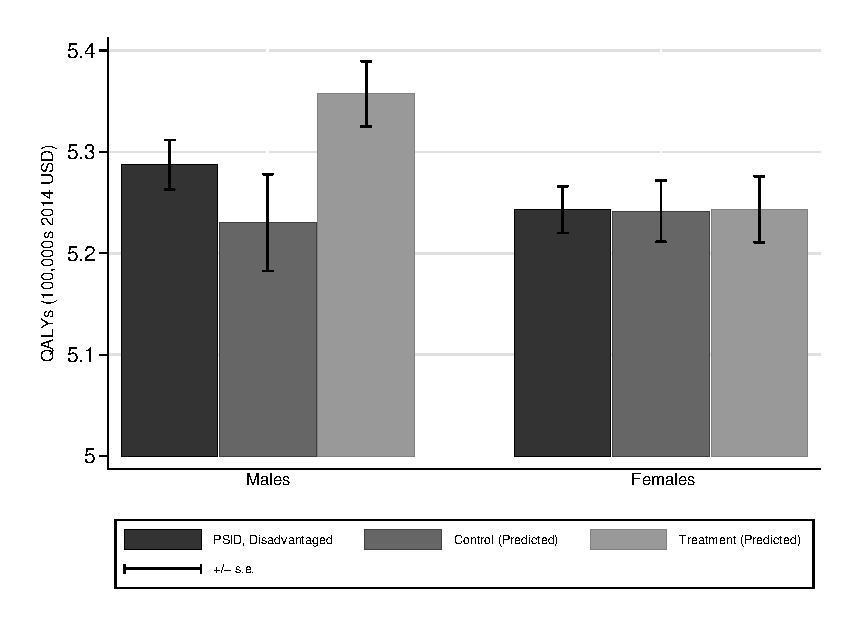
\includegraphics[width=.7\columnwidth]{output/qalyexppsid.eps}
\floatfoot{
\footnotesize
Note:  This figure displays the life-cycle net present value of forecasted quality-adjusted life years (QALYs) for ABC/CARE males and females in the control group. The forecasts are based on combining data from the Panel Study of Income Dynamics (PSID), the Health Retirement Study (HRS), and the Medical Expenditure Panel Survey (MEPS). For each gender, we display a comparison to disadvantaged males and females in the PSID, where disadvantaged is defined as being African American and having at most 12 years of education. QALYs are the quality-adjusted life years accounting for the burden of disease. The black dots indicate that the bars are significantly greater than 0 at the 10\% level. This is calculated using the empirical bootstrap distribution.}
\end{figure}

The same procedure is applied to calculate quality-adjusted life years (QALYs). We compute a QALY model based on a widely-used health-related Quality-of-Life (HRQoL) measure (EQ-5D), available in MEPS.\footnote{For a definition and explanation of this instrument, see \citet{Dolan_1997_Modeling_MC,Shaw_etal_2005_EQ5D_MC}.} We then estimate this model using the PSID.

We estimate three models of medical spending: (i) Medicare spending (annual medical spending paid by parts A, B, and D of Medicare); (ii) private spending (medical spending paid by a private insurer or paid out-of-pocket by the individual); and (iii) all public spending other than Medicare. Each medical spending model includes the variables we use to forecast labor and transfer income, together with current health, risk factors, and functional status as explanatory variables.

We also calculate medical expenditure before age 30 (see Appendix~\ref{appendix:health-costs-before-age30}). The ABC/CARE interviews at ages 12, 15, 21 and 30 have information related to hospitalizations at different ages and number of births before age 30. We combine this information along with individual and family demographic variables to use MEPS to forecast medical spending for each age.

QALYs are crucial for our cost/benefit analysis because they monetize the health of an individual at each age. Figure~\ref{fig:qalys} plots our estimates of mean QALYs together with a PSID comparison for the control sample in an exercise analogous to that used to produce Figure~\ref{fig:labor-income-profiles}.\footnote{In our baseline estimation, we assume that each year of life is worth  $\$150,000$ (2014 USD). Our estimates are robust to substantial variation in this assumption, as we show in  Appendix~\ref{appendix:sensitivity}.} Although there is not a clear age-by-age treatment effect on QALYs, there is a statistically and substantively significant difference in the accumulated present value of the QALYs between the treatment and the control groups. The QALYs for female individuals in the control group match the QALYs of disadvantaged individuals in the PSID. For males, use of the PSID auxiliary sample to construct controls understates the net benefits of ABC/CARE.\footnote{In  Appendix~\ref{appendix:health} we further discuss and justify the parameterizations required to obtain estimates of QALYs. We only consider QALYs starting at age 30. \citet{Goldman_etal_2015_Future-America-Model} examine the sensitivity to these parameterizations and discuss alternative micro-simulations monetizing health condition.}

\subsection{Forecasting Parental Labor Income} \label{section:pincome}

ABC/CARE offers childcare to the parents of treated children for more than nine hours a day for five years, 50 weeks a year. Only $27\%$ of mothers of children reported living with a partner at baseline and this status barely changed during the course of the experiment (see Appendix~\ref{appendix:background}). The childcare component generates substantial treatment effects on maternal labor force participation and parental labor income as reported in \cite{Garcia_Heckman_Ziff_2017_Gender-Diff_UNPUBLISHED}. This arises from wage growth due to parental educational attainment and more work experience.\footnote{There is also an effect on maternal school enrollment. Some of the mothers decided to further enroll in school, obtained a higher degree, and that could be one of the reasons why they make more money afterward. We report these treatment effects in Appendix~\ref{appendix:background}. We quantify the cost of this additional education using the strategy in Appendix~\ref{appendix:education}.}

We observe parental labor income at eight different ages for the experimental subjects up through age 21.\footnote{The ages at which parental labor income is observed are 0, 1.5, 3.5, 4.5, 8, 12, 15, and 21. At age 21 the mothers of the ABC/CARE subjects were, on average, 41 years old.}$^,$\footnote{We linearly interpolate parental labor income for ages for which we do not have observations between 0 and 21.} An ideal approach would be to estimate the profile over the full life-cycle of mothers. We propose two different approaches for doing this in Appendix~\ref{app:parentalincome}: (i) an approach based on parameterizing parental labor income using standard Mincer equations; and (ii) an approach based on the analysis of Section~\ref{section:just}. In Section~\ref{section:cbaresults}, we present estimates using the labor income through age 21 and using these two alternatives for projecting future labor income after age 21. The benefits of the program increase when considering the full life-cycles of mothers using either approach.

Any childcare inducements of the program likely benefit parents who, at baseline, did not have any other children. If they did, then they might have had to take care of other children anyway, weakening the childcare-driven effect, especially if there are younger siblings present. In Appendix~\ref{app:parentalincome}, we show that the treatment effect for discounted parental labor income is much higher when there are no siblings of the participant children at baseline. The effect also weakens when comparing children who have siblings younger than 5 years old to children who have siblings 5 years old or older.\footnote{These patterns persist when splitting the ABC/CARE sample by gender, but the estimates are not precise because the samples become too small. See Appendix~\ref{app:parentalincome}.}

\subsection{Crime}\label{sec:crime}

To estimate the life-cycle benefits and costs of ABC/CARE related to criminal activity, we use rich data on crime outcomes obtained from public records.\footnote{Two previous studies consider the impacts of ABC on crime: \citet{Clarke_Campbell_1998_ABC_Comparison_ECRQ} use administrative crime records up to age 21, and find no statistically significant differences between the treatment and the control groups. \cite{Barnett_Masse_2002_benefitcost,Barnett_Masse_2007_EER} account for self-reported crime at age 21. They find weak effects based on self-reports, but they lack access to longer term, administrative data. The novelty of our study with respect to crime does not only consist of using administrative data allowing us to know the accumulated number of crimes that the children commit once they were in their mid 30s. It is also novel because we use micro-data specific to the state in which these individuals grew up, as well as other national datasets, to forecast criminal activity from the mid 30s to 50.} See Appendix~\ref{appendix:crime} for a more complete discussion. We consider the following types of crime: arson, assault, burglary, fraud, larceny, miscellaneous (which includes traffic and non-violent drug crimes which can lead to incarceration), murder, vehicle theft, rape, robbery, and vandalism. We use administrative data that document: (i) youth arrests, gathered at the age-21 follow-up; (ii) adult arrests, gathered at the mid 30s follow-up; and (iii) sentences, gathered at the mid 30s follow-up. We also use self-reported data on adult crimes, gathered in the age-21 and age-30 subject interviews. Because none of these sources capture all criminal activity, it is necessary to combine them to more completely approximate the crimes the subjects committed. We also use several auxiliary datasets to complete the life-cycle profile of criminal activity and compute the costs of the committed crimes (see Appendix~\ref{appendix:crime-data-description}).

We follow four steps to estimate the costs of crime.

\begin{enumerate}
\item \textit{Count arrests and sentences.} We start by counting the total number of sentences for each individual and type of crime (arson, assault, etc.) up to the mid 30s, matching crimes across data sources, to construct the total number of  arrests for each individual and type of crime up to the mid 30s.\footnote{In practice, we count all offenses (an arrest might include multiple offenses). This gives the correct number of victims for our estimations. The youth data have coarser categories than the rest of the data: violent, property, drug, and other. To match these data with the adult data, we assume that all property crimes were larcenies and that all violent crimes are assaults. In the ABC/CARE sample, assault is the most common type of violent crime, and larceny/theft is the most common property crime.} For individuals missing arrest data,\footnote{About 10\% of the ABC/CARE sample has missing arrest data. We fail to reject the null hypothesis of no differences in observed characteristics between the treatment- and control-group participants for whom we observe arrests data (see  Appendix~\ref{appendix:data}).} we impute the number of arrests by multiplying the number of sentences for each type of crime by a national arrest-sentence ratio for the respective crime.\footnote{This arrest-sentence ratio is constructed using the National Crime Victimization Survey (NJRP) and the Uniform Crime Reporting Statistics (UCRS).}

\item \textit{Construct forecasts.} Based on the sentences observed before the mid 30s, we forecast the sentences that the ABC/CARE subjects will have after their mid 30s. Data from the North Carolina Department of Public Safety (NCDPS), which provide life-cycle sentences of individuals in North Carolina, are used to estimate sentences incurred after the mid 30s from sentences incurred before then. Applying these models to the ABC/CARE data, we forecast the number of future sentences for each subject up to age 50.\footnote{We assume that individuals with no criminal records before their mid 30s commit no crimes thereafter.} We then add these estimates to the original number of sentences, getting an estimate of the life-cycle sentences. Adding these estimates increases the total count of crimes by 30\%--50\%.

\item \textit{Estimate number of victims from the crimes.} We only observe crimes that resulted in consequences in the justice system: crimes that resulted in arrests and/or sentences. To include unobserved crimes, we use victimization inflation (VI).\footnote{Previous papers using this method include \citet{Belfield_Nores_etal_2006_JHR} and \cite{Heckman_Moon_etal_2010_RateofReturn}.} We start by constructing a VI ratio, which is the national ratio of victims to arrests for each type of crime.\footnote{We assume that each crime with victims is counted separately in the national reports on arrests, even for arrests that might have been motivated by more than one crime. This victim-arrest ratio is constructed using the NJRP and the National Crime Victimization Survey (NCVS).} Then, we estimate the number of victims from the crimes committed by ABC/CARE subjects as their total arrests multiplied by the VI ratio.\footnote{Additionally, we can calculate an analogous estimate of the number of crime victims using sentences, based on the VI ratio and the national arrest-sentence ratio. These estimates are very similar, as shown in Appendix~\ref{appendix:crime-VI}. To improve precision, the estimates in the rest of our paper are based on the average of the two calculations.}

\item \textit{Find total costs of crimes.} We use the estimates of the cost of crimes for victims from \cite{McCollister_etal_2010_DAD} to impute the total victimization costs. For crimes resulting in arrests and/or sentences, we consider criminal justice system costs as well, such as police costs.\footnote{To be able to assign costs to each type of crime, we assume that the cost of the justice system depends on the number of offenses of each type, rather than on the number of arrests. While this could very slightly overestimate justice system costs, these costs only represent about 5\% of the total crime costs.} Finally, we construct the total costs of incarceration for each subject using the total prison time and the cost of a day in prison.\footnote{ Appendix~\ref{appendix:sensitivity} examines the sensitivity of our crime costs quantification to different assumptions. Section~\ref{section:cbaresults} and  Appendix~\ref{appendix:sensitivity} examine the sensitivity of our overall assessment of ABC/CARE results to the quantification of crime that we explain in this section.}
\end{enumerate}

\subsection{Program Costs} \label{section:programscosts}

The yearly cost of the program was \$18,514 per participant in 2014 USD. We improve on previous cost estimates using primary-source documents.\footnote{Our calculations are based on progress reports written by the principal investigators and related documentation recovered in the archives of the research center where the program was implemented. We display these sources in Appendix~\ref{app:programcosts}. The main component is staff costs. Other costs arise from nutrition and services that the subjects receive when they were sick, diapers during the first 15 months of their lives, and transportation to the center. The control-group children also receive diapers during approximately 15 months, and iron-fortified formula. The costs are based on sources describing ABC treatment for $52$ children. We use the same costs estimates for CARE, for which there is less information available. The costs exclude any expenses related to research or policy analysis. A separate calculation by the implementers of the program indicates almost an identical amount (see  Appendix~\ref{app:programcosts}).} Appendix~\ref{app:programcosts} discusses the program costs in detail. This section reports benefit/cost and rate of return analyses underlying Figure~\ref{figure:main}.  Appendix~\ref{appendix:sensitivity} displays an extensive sensitivity analysis of each of the components we consider. It includes scenarios in which all of our assumptions hold and scenarios in which they are violated, providing bounds for our estimates.

\section{Estimating the Benefit/Cost Ratio and the Internal Rate of Return} \label{section:cbaresults}

We first present our main estimates and then conduct sensitivity analyses.\footnote{See Appendices~\ref{app:method_irr} and~\ref{app:method_cbratio} for more details on these estimations. We note that one limitation of our analysis is that data limitations prevent us from jointly estimating all of the behavioral relationships considered in this paper. Different components of the net benefits are estimated on different data sets.} Table~\ref{table:bcsens} gives our baseline estimates of benefit/cost ratios and the sensitivity of the estimates to alternative assumptions. Table~\ref{table:irrsens} presents the corresponding internal rates of return. Pooling males and females, the results indicate that the program is socially efficient: the internal rate of return and the benefit/cost ratio are $13.7\%$ and $7.3$. \textit{Our baseline estimates indicate that the program generates a benefit of $7.3$ dollars for every dollar spent on it}. These estimates are statistically significant, even after accounting for sampling variation, serial correlation, and forecast error in the experimental and auxiliary samples and the tax costs of financing the program.\footnote{We obtain the reported standard errors by bootstrapping \emph{all} steps of our empirical procedure, including variable selection, imputation, model selection steps, and forecast error (see  Appendix~\ref{appendix:bootstrap}).} These benefits arise despite the fact that ABC/CARE was much more expensive than other early childhood education programs because the program used more services over a longer time period.

We accompany these estimates with an extensive set of sensitivity checks of statistical and economic interest. Our estimates are not driven by our methods for accounting for attrition and item non-response, by the conditioning variables, or the functional forms of projection equations used when computing the net-present values.\footnote{See Appendix~\ref{appendix:methodology} for a detailed discussion.} Although the internal rate of return remains relatively high when using participant outcome measures only up to ages 21 or 30, the benefit/cost ratios indicate that accounting for benefits that go beyond age 30 is important. The return to each dollar is at most $3/1$ when only considering benefits up to age 30 only (forecast span columns). Accounting for the treatment substitutes available to controls also matters. Males benefit the most from ABC/CARE relative to attending alternative childcare, while females benefit the most from ABC/CARE relative to staying at home. We explore this difference below.

\begin{sidewaystable}[!htpb]
\begin{threeparttable}
\caption{Sensitivity Analysis for Benefit/Cost Ratios}
\label{table:bcsens}
\centering
\scriptsize
\begin{tabular}{>{\bfseries}lcc|cc|cc} \toprule
	&	\multicolumn{2}{c}{\textbf{\textit{Pooled}}}	&	\multicolumn{2}{c}{\textbf{\textit{Males}}}	&	\multicolumn{2}{c}{\textbf{\textit{Females}}}	\\ 
Baseline	&	\multicolumn{2}{c}{5.69 (s.e. 2.32)}	&	\multicolumn{2}{c}{11.62 (s.e. 5.49)}	&	\multicolumn{2}{c}{2.60 (s.e. 0.98)}	\\ \\
\multicolumn{7}{l}{\textit{Baseline: IPW and Controls, Life-span up to Age 79, Treatment vs. Next Best, 50\% Marginal tax 50\% (deadweight loss), Discount rate 3\%, Parental}} \\	
\multicolumn{7}{l}{\textit{income 0 to 21 (child's age), Labor Income predicted from 21 to 65, All crimes (full costs), Value of life 150,000.}} \\ \\ \midrule	
Specification	&	\textit{No IPW}	&	\textit{and No Controls}	&	\textit{No IPW}	&	\textit{and No Controls}	&	\textit{No IPW}	&	\textit{and No Controls}	\\
	&	\textbf{6.17}	&	\textbf{5.35}	&	\textbf{11.94} 	&	\textbf{10.74}	&	\textbf{2.91}	&	\textbf{2.79}	\\
	&	(2.35)	&	(2.04)	&	(6.14)	&	(4.12)	&	(0.97)	&	(0.81)	\\ \midrule
Prediction	&	\textit{to Age 21}	&	\textit{to Age 30}	&	\textit{to Age 21}	&	\textit{to Age 30}	&	\textit{to Age 21}	&	\textit{to Age 30}	\\
Span	&	\textbf{1.55}	&	2.01	&	\textbf{2.17}	&	2.80	&	1.17	&	1.52	\\
	&	(0.39)	&	(0.88)	&	(0.74)	&	(1.96)	&	(0.43)	&	(0.48)	\\ \midrule
Counter-	&	\textit{vs. Stay at Home}	&	\textit{vs. Alt. Presch.}	&	\textit{vs. Stay at Home}	&	\textit{vs. Alt. Presch.}	&	\textit{vs. Stay at Home}	&	\textit{vs. Alt. Presch.}	\\
factuals	&	\textbf{4.44}	&	\textbf{6.58}	&	3.88	&	\textbf{10.85}	&	\textbf{4.89}	&	\textbf{2.40}	\\
	&	(1.68)	&	(2.22)	&	(2.78)	&	(4.14)	&	(1.50)	&	(0.94)	\\ \midrule
Deadweight-	&	\textit{0\%}	&	\textit{100\%\textit}	&	\textit{0\%}	&	\textit{100\%\textit}	&	\textit{0\%}	&	\textit{100\%\textit}	\\
loss	&	\textbf{8.50}	&	\textbf{4.29}	&	\textbf{17.43}	&	\textbf{8.71}	&	\textbf{3.69}	&	2.06	\\
	&	(3.47)	&	(1.75)	&	(8.19)	&	(4.14)	&	(1.43)	&	(0.79)	\\ \midrule
Discount 	&	\textit{0\%}	&	\textit{7\%}	&	\textit{0\%}	&	\textit{7\%}	&	\textit{0\%}	&	\textit{7\%}	\\
Rate	&	13.38	&	2.40	&	29.50	&	4.21	&	5.34	&	1.43	\\
	&	7.01	&	0.80	&	15.93	&	1.88	&	3.81	&	0.37	\\ \midrule
Parental	&	\textit{Mincer Life-cycle}	&	\textit{Life-cycle Prediction}	&	\textit{Mincer Life-cycle}	&	\textit{Life-cycle Prediction}	&	\textit{Mincer Life-cycle}	&	\textit{Life-cycle Prediction}	\\
Income	&	\textbf{5.92}	&	\textbf{5.60}	&	\textbf{11.80}	&	\textbf{12.36}	&	\textbf{2.88}	&	\textbf{3.27}	\\
	&	(2.32)	&	(2.39)	&	(5.49)	&	(5.68)	&	(1.02)	&	(1.21)	\\ \midrule
Labor	&	\textit{.5\% Annual Decay}	&	\textit{.5\% Annual Growth}	&	\textit{.5\% Annual Decay}	&	\textit{.5\% Annual Growth}	&	\textit{.5\% Annual Decay}	&	\textit{.5\% Annual Growth}	\\
Income	&	\textbf{5.48}	&	\textbf{5.90}	&	\textbf{10.76}	&	\textbf{12.49}	&	\textbf{2.47}	&	\textbf{2.74}	\\
	&	(2.25)	&	(2.41)	&	(5.33)	&	(5.71)	&	(0.87)	&	(1.10)	\\ \midrule
Crime	&	\textit{Drop Major Crimes}	&	\textit{Halve Costs}	&	\textit{Drop Major Crimes}	&	\textit{Halve Costs}	&	\textit{Drop Major Crimes}	&	\textit{Halve Costs}	\\
	&	\textbf{5.14} 	&	\textbf{4.07}	&	\textbf{11.82}	&	\textbf{8.33}	&	\textbf{2.72}	&	2.25	\\
	&	(2.30)	&	(1.50)	&	(5.59)	&	(3.64)	&	(1.04)	&	(0.95)	\\ \midrule
Health	&	\textit{Drop All}	&	\textit{Double Value of Life}	&	\textit{Drop All}	&	\textit{Double Value of Life}	&	\textit{Drop All}	&	\textit{Double Value of Life}	\\
(QALYs)	&	\textbf{4.85}	&	\textbf{6.56}	&	\textbf{10.61}	&	\textbf{12.63}	&	\textbf{2.48}	&	2.73	\\
	&	(2.32)	&	(2.54)	&	(5.37)	&	(5.90)	&	(0.97)	&	(1.26)	\\ \bottomrule
\end{tabular} 
\begin{tablenotes}
\scriptsize
\item Note: This table displays sensitivity analyses of our baseline benefit/cost ratio calculation to the perturbations indexed in the different rows. The characteristics of the \textit{baseline} calculation are in the table header. IPW: adjusts for attrition and item non-response (see  Appendix~\ref{app:method_partialobs} for details). Control variables: Apgar scores at ages 1 and 5 and a high-risk index (see  Appendix~\ref{appendix:results} for details on how we choose these controls). When forecasting up to ages 21 and 30, we consider all benefits and costs up to these ages, respectively. Counterfactuals: we consider treatment vs. next best (baseline), treatment vs. stay at home, and treatment vs. alternative preschools (see Section~\ref{section:methodsquestions} for a discussion). Deadweight loss is the loss implied by any public expenditure (0\% is no loss and 100\% is one dollar loss per each dollar spent). Discount rate: rate to discount benefits to child's age 0 (in all calculations). Parental labor income: see  Appendix~\ref{app:parentalincome} for details on the two alternative forecasts (Mincer and Life-cycle). Labor Income: 0.5\ annual growth (decay) is an annual wage growth (decay) due to cohort effects. Crime: major crimes are rape and murder; half costs takes half of victimization and judiciary costs. Health (QALYs): ``drop all'' sets the value of life equal to zero. Standard errors obtained from the empirical bootstrap distribution are in parentheses. Bolded $p$-values are significant at 10\% using one-sided tests. For details on the null hypothesis see Table~\ref{table:cba}.
\end{tablenotes}
\end{threeparttable}
\end{sidewaystable}

\begin{sidewaystable}[!htpb]
\begin{threeparttable}
\caption{Sensitivity Analysis for Internal Rate of Return, ABC/CARE}
\label{table:irrsens}
\centering
\scriptsize
% matrix: allirr file: allirr_sens.tex  25 Sep 2016 09:11:16
\begin{table}[htbp]
\begin{tabular}{lcccccc} \hline \hline
 & pooled  & pooled  & males  & males  & females  & females  \\  \hline 
baseline &     0.087 &     0.052 &     0.138 &     0.048 &     0.126 &     0.048 \\  
specification &     0.092 &     0.087 &     0.147 &     0.148 &     0.136 &     0.122 \\  
. &     0.059 &     0.032 &     0.060 &     0.037 &     0.044 &     0.039 \\  
predictiontime &     0.099 &     0.127 &     0.110 &     0.127 &     0.104 &     0.115 \\  
. &     0.056 &     0.051 &     0.047 &     0.051 &     0.045 &     0.043 \\  
counterfactual &     0.131 &     0.089 &     0.085 &     0.162 &     0.100 &     0.132 \\  
. &     0.046 &     0.057 &     0.038 &     0.044 &     0.034 &     0.039 \\  
dwl &     0.128 &     0.068 &     0.175 &     0.118 &     0.174 &     0.103 \\  
. &     0.089 &     0.037 &     0.063 &     0.042 &     0.064 &     0.037 \\  
parental &     0.104 &         . &     0.148 &         . &     0.142 &         . \\  
. &     0.069 &         . &     0.053 &         . &     0.053 &         . \\  
lincome &     0.080 &         . &     0.127 &         . &     0.122 &         . \\  
. &     0.053 &         . &     0.054 &         . &     0.047 &         . \\  
crime &     0.089 &     0.081 &     0.153 &     0.122 &     0.124 &     0.110 \\  
. &     0.052 &     0.051 &     0.043 &     0.046 &     0.044 &     0.044 \\  
health &     0.091 &     0.085 &     0.136 &     0.134 &     0.112 &     0.127 \\  
. &     0.053 &     0.052 &     0.049 &     0.053 &     0.058 &     0.045 \\  
\hline \hline \end{tabular}
\end{table}

\begin{tablenotes}
\scriptsize
\item Note: This table displays sensitivity analyses of our baseline internal rate of return calculation to the perturbations indexed in the different rows. The characteristics of the \textit{baseline} calculation are in the table header. IPW: adjusts for attrition and item non-response (see  Appendix~\ref{app:method_partialobs} for details). Control variables: Apgar scores at ages 1 and 5 and a high-risk index (see  Appendix~\ref{appendix:results} for details on how we choose these controls). When forecasting up to ages 21 and 30, we consider all benefits and costs up to these ages, respectively. Counterfactuals: we consider treatment vs. next best (baseline), treatment vs. stay at home, and treatment vs. alternative preschools (see Section~\ref{section:methodsquestions} for a discussion). Deadweight loss is the loss implied by any public expenditure (0\% is no loss and 100\% is one dollar loss per each dollar spent). Parental labor income: see  Appendix~\ref{app:parentalincome} for details on the two alternative forecasts (Mincer and Life-cycle). Labor Income: 0.5\ annual growth is an annual wage growth due to cohort effects; only benefit assumes labor income is the only benefit of the program. Crime: major crimes are rape and murder; half costs takes half of victimization and judiciary costs. Health (QALYs): ``drop all'' sets the value of life equal to zero. Bolded $p$-values are significant at 10\% using one-sided tests. For details on the null hypothesis see Table~\ref{table:cba}.
\end{tablenotes}
\end{threeparttable}
\end{sidewaystable}
\doublespacing

Our baseline estimates account for the deadweight loss caused by distortionary taxes to fund programs, plus the direct costs associated with collecting taxes.\footnote{When the transaction between the government and an individual is a direct transfer, we consider 0.5 as the cost per each transacted dollar. We do not weight the final recipient of the transaction (e.g., transfer income). When the transaction is indirect, we classify it as government spending as a whole and consider its cost as 1.5 per each dollar spent (e.g., public education).} We assume a marginal tax rate of $50\%$.\footnote{\citet{Feldstein_1999_REStat} reports that the deadweight loss caused by increasing existing tax rates (marginal deadweight loss) may exceed two dollars per each dollar of revenue generated. We use a more conservative value (0.5 dollars per each dollar of revenue generated). In Tables~\ref{table:bcsens}, \ref{table:irrsens}, and \ref{table:cba} and in  Appendix~\ref{appendix:varying-dwl}, we explore the robustness of this decision and find little sensitivity.} Our estimates are robust to dropping it to $0\%$ or doubling it to $100\%$ (deadweight loss columns). Our baseline estimate of benefit/cost ratios is based on a discount rate of $3\%$. Not discounting roughly doubles our benefit/cost ratios, while they remain statistically significant using a higher discount rate of $7\%$ (discount rate columns).

Parental labor income effects induced by the childcare subsidy is an important component of the benefit/cost ratio. We take a conservative approach in our baseline estimates and do not account for potential shifts in profiles in parental labor income due to education and work experience subsidized by childcare (see the discussion in Section~\ref{section:pincome}). Our baseline estimates rely solely on parental labor income when participant children are ages 0 to 21. Alternative approaches considering the gain for the parents through age 67 generate an increase in the gain due to parental labor income (see parental labor income columns).

As noted in Section~\ref{section:cbamethodology}, the baseline estimates ignore cohort effects. Individuals in ABC/CARE could experience positive cohort effects that might (i) make them more productive and therefore experience wage growth \citep{Lagakos_Moll_etal_2016_LifeCycle_NBER}; (ii) experience a negative shock such as an economic crisis and therefore experience a wage decline \citep{Jarosch_2016_JobSecurity_Econometrica}. Our estimates are robust when we vary annual growth and decay rates between $-0.5\%$ and $0.5\%$.\footnote{We account for cohort effects in health as explained in Section~\ref{section:health}.}

\begin{table}[H]
\centering
\caption{Cost/Benefit Analysis of ABC/CARE, Summary}\label{table:cba}
\begin{threeparttable}
\tiny
\begin{tabular}{l r r r r r r r r r}																			
\toprule																			
&       \mc{3}{c}{Females}      &       \mc{3}{c}{Males}        &       \mc{3}{c}{Pooled}       \\																			
\cmidrule(lr){2-4}      \cmidrule(lr){5-7}      \cmidrule(lr){8-10}																			
Removed Component       &       NPV     &       IRR     &       B/C     &       NPV     &       IRR     &       B/C     &       NPV     &       IRR     &       B/C     \\																			
\midrule																			
None	&	161,759	&	\textbf{10.1\%}	&	\textbf{2.61}	&	919,049	&	\textbf{14.7\%}	&	\textbf{10.19}	&	636,674	&	\textbf{13.7\%}	&	\textbf{7.33}	\\
	&		&	(6\%)	&	(0.73)	&		&	(4\%)	&	(2.93)	&		&	(3\%)	&	(1.84)	\\ \\
Parental Income	&	148,854	&	4\%	&	1.12	&	107,907	&	\textbf{11\%}	&	\textbf{9.10}	&	116,953	&	\textbf{9\%}	&	\textbf{6.17}	\\
	&		&	(2\%)	&	(0.65)	&		&	(3\%)	&	(2.92)	&		&	(3\%)	&	(1.87)	\\
Subject Labor Income	&	41,908	&	9\%	&	\textbf{2.21}	&	238,105	&	\textbf{13\%}	&	\textbf{7.75}	&	133,032	&	\textbf{13\%}	&	\textbf{6.03}	\\
	&		&	(6\%)	&	(0.66)	&		&	(5\%)	&	(2.23)	&		&	(4\%)	&	(1.77)	\\
Subject Transfer Income	&	419	&	\textbf{10\%}	&	\textbf{2.61}	&	-7,265	&	\textbf{15\%}	&	\textbf{10.26}	&	-4,372	&	\textbf{14\%}	&	\textbf{7.38}	\\
	&		&	(6\%)	&	(0.73)	&		&	(4\%)	&	(2.93)	&		&	(3\%)	&	(1.84)	\\
Subject QALY	&	42,102	&	9\%	&	\textbf{2.20}	&	106,218	&	\textbf{14\%}	&	\textbf{9.14}	&	87,181	&	\textbf{13\%}	&	\textbf{6.48}	\\
	&		&	(6\%)	&	(0.69)	&		&	(6\%)	&	(2.73)	&		&	(5\%)	&	(1.79)	\\
Medical Expenditures	&	-16,037	&	9\%	&	\textbf{2.77}	&	-42,038	&	\textbf{15\%}	&	\textbf{10.61}	&	-31,221	&	\textbf{14\%}	&	\textbf{7.65}	\\
	&		&	(6\%)	&	(0.76)	&		&	(3\%)	&	(2.89)	&		&	(3\%)	&	(1.85)	\\
Alternative Preschools	&	16,691	&	8\%	&	\textbf{2.45}	&	13,434	&	\textbf{14\%}	&	\textbf{10.05}	&	14,659	&	\textbf{12\%}	&	\textbf{7.19}	\\
	&		&	(5\%)	&	(0.73)	&		&	(4\%)	&	(2.92)	&		&	(3\%)	&	(1.84)	\\
Education Costs	&	1,457	&	\textbf{10\%}	&	\textbf{2.59}	&	-7,852	&	\textbf{15\%}	&	\textbf{10.26}	&	-4,518	&	\textbf{14\%}	&	\textbf{7.37}	\\
	&		&	(6\%)	&	(0.72)	&		&	(4\%)	&	(2.93)	&		&	(3\%)	&	(1.86)	\\
Crime Costs	&	31,668	&	10\%	&	\textbf{2.34}	&	638,923	&	\textbf{9\%}	&	4.08	&	450,368	&	\textbf{8\%}	&	\textbf{3.06}	\\
	&		&	(6\%)	&	(0.62)	&		&	(5\%)	&	(2.18)	&	&	(4\%)	&	(1.01)	\\ \\
Deadweight Loss	&		&	\textbf{18\%}	&	\textbf{3.83}	&		&	\textbf{19\%}	&	\textbf{15.38}	&		&	\textbf{18\%}	&	\textbf{11.01}	\\
	&		&	(12\%)	&	(1.04)	&		&	(6\%)	&	(4.35)	&		&	(5\%)	&	(2.79)	\\
0\% Discount Rate	&		&		&	\textbf{5.06}	&		&		&	\textbf{25.45}	&		&		&	\textbf{17.40}	\\
	&		&		&	(2.82)	&		&		&	(10.42)	&		&		&	(5.90)	\\
7\% Discount Rate	&		&		&	\textbf{1.49}	&		&		&	\textbf{3.78}	&		&		&	\textbf{2.91}	\\
	&		&		&	(0.32)	&		&		&	(0.79)	&		&		&	(0.59)	\\
\bottomrule																			
\end{tabular}																			

\begin{tablenotes}
\footnotesize
\item Note: This table presents the estimates of the net present value (NPV) for each component, and the internal rate of return (IRR) and the benefit/cost ratio (B/C) of ABC/CARE for different scenarios based on comparing the groups randomly assigned to receive center-based childcare and the groups randomly assigned as control in ABC/CARE. The first row represents the baseline estimates. The other rows present estimates for scenarios in which we remove the NPV estimates of the component listed in the first column. The category ``Alternative Preschools'' refers to the money spent in alternatives to treatment from the control-group children parents. QALYs refers to the quality-adjusted life years. Any gain corresponds to better health conditions through the age of death. The quantity listed in the NPV columns is the component we remove from NPV when computing the calculation in each row. All the money figures are in 2014 USD and are discounted to each child's birth, unless otherwise specified. For the B/C ratio we use a discount rate of $3\%$, unless otherwise specified. We test the null hypotheses $\text{IRR} = 3\%$ and $\text{B/C} = 1$---we select $3\%$ as the benchmark null because that is the discount rate we use. Inference is based on non-parametric, one-sided $p$-values from the empirical bootstrap distribution. We highlight point estimates significant at the $10\%$ level. Total cost of the program per child is \$$92,570$ (2014).
\end{tablenotes}
\end{threeparttable}
\end{table}

We also examine the sensitivity of our estimates to (i) dropping the most costly crimes such as murders and rapes;\footnote{Two individuals in the treatment group were convicted of rape and one individual in the control group was convicted of murder.} and (ii) halving the costs of victimization and judiciary costs related to crime. The first sensitivity check is important because we do not want our estimates to be based on a few exceptional crimes. The second is important because victimization costs are somewhat subjective (see  Appendix~\ref{appendix:crime-VI}). Our cost/benefit estimates are robust to these adjustments, even though crime is a major component of it. We also examine the sensitivity with respect to our main health component: quality-adjusted life years. This is an important component because healthier individuals survive longer, and treatment improves health conditions. It is important to note that this component largely accumulates later in life and therefore is heavily discounted. Dropping the component or doubling the value of life does not have a major impact on our calculations.

The estimates are robust when we conduct a rather drastic sensitivity analysis by removing components of the cost/benefit analysis entirely (see Table~\ref{table:cba} and Figure~\ref{figure:vennpooled}).\footnote{In  Appendix~\ref{app:sa_factors}, we present exercises that are not as drastic as removing the whole component, but instead remove fractions of it.} Even when completely removing the gain associated with crime for males, the program is socially efficient---both the internal rate of return and the benefit/cost ratio are substantial. Parental labor income and crime are the components for which the internal rate of return and the benefit/cost ratio are the most sensitive. The reason for this sensitivity to parental labor income is that the amount is substantial and it is not heavily discounted because it accumulates during the first $21$ years of the subjects' lives. Crime occurs later in life and its benefits are discounted accordingly. The amount due to savings in crime is large, so removing it diminishes both the internal rate of return and the benefit/cost ratio (but they remain statistically significant).

In  Appendix~\ref{appendix:predsensitivity}, we investigate how sensitive our forecast model is to a variety of perturbations: different autocorrelation processes in the forecast errors, functional forms of the prediction equations, forecasts without lagged variables, etc. Our estimates are robust to using different forecast models.

\textit{Overall, our sensitivity analyses indicate that no single category of outcomes drives the social efficiency of the program (see Figures~\ref{figure:vennpooled} and \ref{figure:ranges}). Rather, it is the life-cycle benefits across multiple dimensions of human development.}

\begin{sidewaysfigure}[!htbp]
\centering
\caption{Life-cycle Net Present Value of Main Components of the CBA}\label{fig:npvsgender}
\begin{subfigure}[h]{0.5\textwidth}
		\centering
		\caption{Males}
		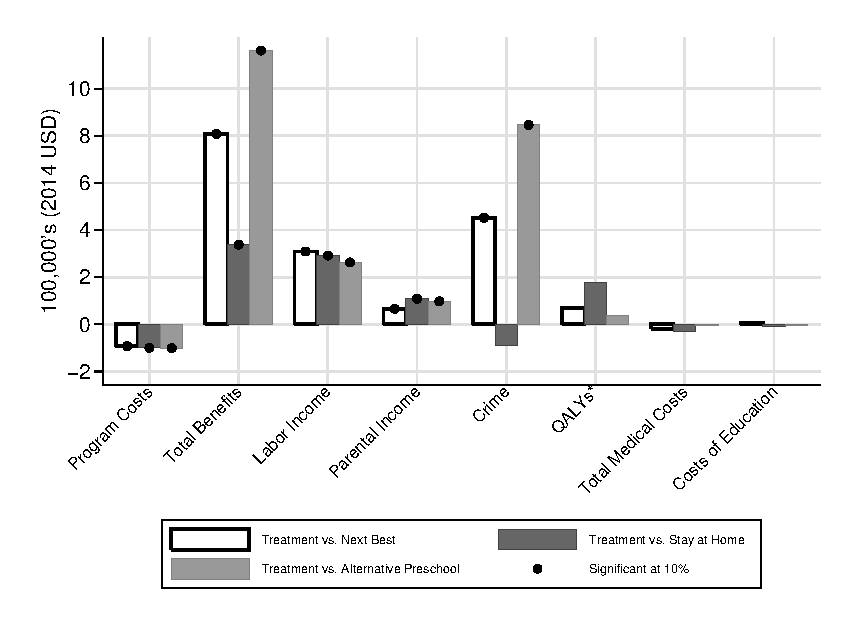
\includegraphics[width=\textwidth]{output/abccare_npvs2.eps}
\end{subfigure}%
\begin{subfigure}[h]{0.5\textwidth}
		\centering
		\caption{Females}
		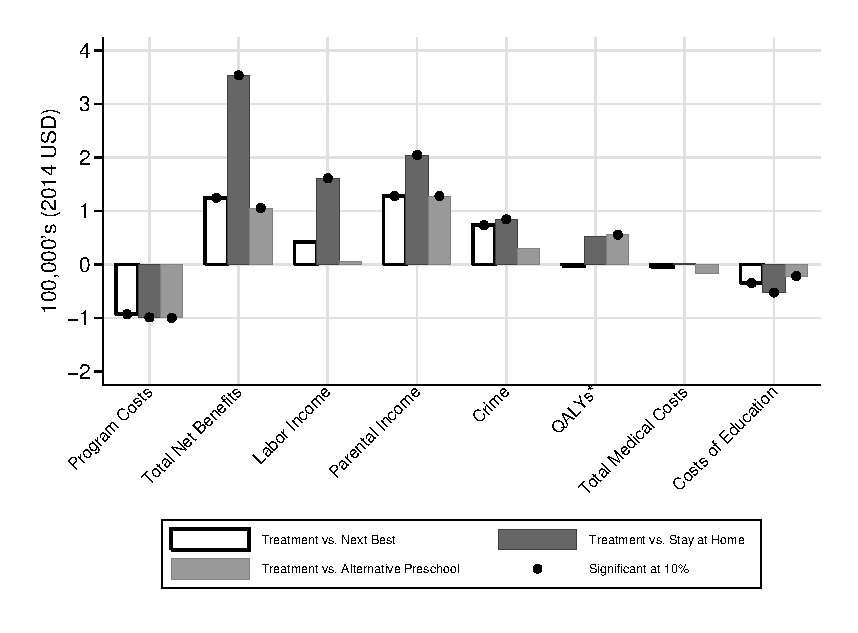
\includegraphics[width=\textwidth]{output/abccare_npvs1.eps}
\end{subfigure}
\scriptsize \justify
Note: This figure displays the life-cycle net present values of the main components of the cost/benefit analysis of ABC/CARE from birth to forecasted death, discounted to birth at a rate of 3\%. ``Treatment vs. Control'': compares the treatment to the control group. ``Treatment vs. Stay at Home'': compares the treatment group to those subjects who stayed at home. ``Treatment vs. Alternative Preschool'': compares the treatment group to those subjects who attended alternative preschools. The latter two are based on matching estimators that account for selection on observable variables. By ``net" we mean that each component represents the total value for the treatment group minus the total value for the control group. Program costs: the total cost of ABC/CARE, including the welfare cost of taxes to finance it. Total net benefits: are for \textit{all} of the components we consider. Labor income: total individual labor income from ages 20 to the retirement of program participants (assumed to be age 67). Parental labor income: total parental labor income of the parents of the participants from when the participants were ages 1.5 to 21. Crime: the total cost of crime (judicial and victimization costs). To simplify the display, the following components are not shown in the figure: (i) cost of alternative preschool paid by the parents of control group children; (ii) the social welfare costs of transfer income from the government; (iii) disability benefits and social security claims; (iv) costs of increased individual and maternal education (including special education and grade retention); (v) total medical public and private costs. Inference is based on non-parametric, one-sided $p$-values from the empirical bootstrap distribution. We indicate point estimates significant at the $10\%$ level.\\
*The treatment vs. stay at home net present value is sizable and negative (-\$123,498,.2); its standard error is \$62,745.72.\\
**QALYs refers to the quality-adjusted life years. Any gain corresponds to better health conditions until forecasted death, with $\$150,000$ (2014 USD) as the base value for a year of life.\\
\end{sidewaysfigure}

\section{Using Our Estimates to Understand Recent Benefit/Cost Analyses}\label{section:bcaestimates}

We use our analysis to examine the empirical foundations of the approach to benefit/cost analysis taken in a prototypical study of \citet{Kline_Walters_2016_QJE}, which in turn is based on estimates taken from \citet{Chetty_Friedman_etal_2011_QJoE}. Although widely emulated, this approach offers an imprecise approximation of benefit/cost ratios with questionable validity. Examples of application of this approach include \citet{Attanasio_Kugler_Meghir_2011_AEJAE}, \cite{Behrman-et-al_2011_JHR-Progresa}, and \cite{Deshpande_Yue_2017_Screened_Unpublished}.

\citet{Kline_Walters_2016_QJE} use data from the Head Start Impact Study (HSIS) and report a benefit/cost ratio between $1.50$ and $1.84$.\footnote{HSIS is a one-year-long randomized evaluation of Head Start.} Their analysis proceeds in three steps: (i) calculate program treatment effects on IQ measured around age 5\footnote{They use an index based on the Peabody Picture Vocabulary and Woodcock Johnson III Tests.}; (ii) monetize this gain using the return to the IQ measured between ages 5 and 7 in terms of net present value of labor income at age 27 using the estimates of \citet{Chetty_Friedman_etal_2011_QJoE}.\footnote{The \citet{Chetty_Friedman_etal_2011_QJoE} return is based on Stanford Achievement Tests.}$^,$\footnote{For this comparison exercise, we interpret the earnings estimated in \citet{Chetty_Friedman_etal_2011_QJoE} to be equivalent to labor income.}$^,$\footnote{Calculations from \citet{Chetty_Friedman_etal_2011_QJoE} indicate that a 1 standard deviation gain in IQ at age 5 implies a $13.1\%$ increase in the net present value of labor income through age 27. This is based on combining information from Project Star and administrative data at age 27.}; and (iii) calculate the benefit/cost ratio based on this gain and their own calculations of the program's cost.\footnote{Their calculation assigns the net present value of labor income through age 27 of $\$385,907.17$ to the control-group participants, as estimated by  \citet{Chetty_Friedman_etal_2011_QJoE}.}$^,$\footnote{All monetary values that we provide in this section are in 2014 USD. We discount the value provided by \citet{Chetty_Friedman_etal_2011_QJoE} to the age of birth of the children in our sample (first cohort).}

\begin{table}[!htbp]
\begin{threeparttable}
\caption{Alternative Cost/Benefit Analyses Calculations}
\label{table:comparing}
\centering
\footnotesize

\begin{tabular}{cllcc}
\toprule
Age & \mc{1}{c}{NPV Source} & Component & \citet{Kline_Walters_2016_QJE} & Authors' Method \\
& & & Method & \\
\midrule
\multirow{2}{*}{27} & \cite{Chetty_Friedman_etal_2011_QJoE} & Labor income & 0.58 (s.e. 0.28) &  \\
& ABC/CARE-calculated & Labor income & 0.09 (s.e. 0.04) &  1.09 (s.e. 0.04)\\
\midrule
\multirow{2}{*}{34} & ABC/CARE-calculated & Labor income & 0.37 (s.e. 0.04) & 0.15 (s.e. 0.05) \\
& ABC/CARE-calculated & All & 1.21 (s.e. 0.05) &  3.20 (s.e. 1.04) \\
\midrule
\multirow{2}{*}{Life-cycle} &  ABC/CARE-calculated & Labor income & 1.56 (s.e. 0.08) & 1.55 (s.e. 0.76) \\
& ABC/CARE-calculated & All & 3.80 (s.e. 0.29) & 7.33 (s.e. 1.84) \\
\bottomrule
\end{tabular}

\begin{tablenotes}
\footnotesize
\item Note: This table displays benefit/cost ratios based on the methodology in \citet{Kline_Walters_2016_QJE} and based on our own methodology. Age: age at which we stop calculating the net present value. NPV Source: source where we obtain the net present value. Component: item used to compute net present value (all refers to the net present value of all the components). \citet{Kline_Walters_2016_QJE} Method: estimate based on these authors' methodology. Authors' Method: estimates based on our methodology. Standard errors are based on the empirical bootstrap distribution.
\end{tablenotes}
\end{threeparttable}
\end{table}

To analyze how our estimates compare to those based on this method, we present a series of exercises in the fourth column of Table~\ref{table:comparing}. For purposes of comparison, the fifth column of Table~\ref{table:comparing} shows the analogous estimates based on our own samples and forecasts.

In the first exercise, we calculate the benefit/cost ratio using both the ``return to IQ'' and the net present value of labor income at age 27 reported in \citet{Chetty_Friedman_etal_2011_QJoE}. This calculation is the same type of calculation as that used in \citet{Kline_Walters_2016_QJE}. In the second exercise, we perform a similar exercise but use our own estimate of the net present value of labor income at age 27.\footnote{This allows us to compute our own ``return to IQ'' and impute it to the treatment-group individuals.} In this exercise, the standard errors account for variation in the return because we calculate the return in every bootstrapped re-sample. In that sense, our approach is a valid account of underlying uncertainties when compared to \citet{Kline_Walters_2016_QJE}, who do not account for estimation error in reporting standard errors. The return is smaller because our sample is much more disadvantaged than that of \citet{Chetty_Friedman_etal_2011_QJoE}.

The remaining exercises are similar, but we (i) increase the age range over which we calculate the net-present value of labor income; or (ii) consider the value of all the components we analyze throughout the paper, in addition to labor income. The more inclusive the benefits measured and the longer the horizon over which they are measured, the greater the benefit/cost ratio. The final reported estimate, 7.33, is our baseline estimate that incorporates all of the components across the life cycle of the subjects.

Our methodology provides a more accurate estimate of the net present value (and the return to IQ) of the program. We better quantify the effects of the experiment by considering benefits over the whole life cycle. We also better approximate the statistical uncertainty of our estimates by considering both the sampling error in the experimental and auxiliary samples and the forecast error due to the interpolation and extrapolation. Proceeding in this fashion enables us to examine the sensitivity of each of the components in our study that we monetize.

\section{Summary} \label{section:conclusion}

This paper goes beyond analyzing batteries of short-term of treatment effects on test scores to evaluate early education programs---a standard practice in the current literature. Based on the large array of treatment effects from ages 0 to mid 30s reported in \citet{Garcia_Heckman_Ziff_2017_Gender-Diff_UNPUBLISHED}, we combine experimental and non-experimental datasets to forecast long-term outcomes. We use these forecasts to compute statistics summarizing the social efficiency of the influential and widely implemented program that we evaluate.

Our analysis accounts for multiple sources of statistical and modeling uncertainty. We go beyond current analyses that only quantify a single, short-term treatment effect to forecast labor income without providing a sense of statistical and modeling uncertainty. We quantify long-term costs and benefits and provide a life-cycle analysis. We quantify and monetize health outcomes, a novel outcome in the evaluation of early childhood programs.

We demonstrate the benefits of economic and econometric theory, and auxiliary data sets, for evaluating the long-term benefits of a social experiment. Our forecasts rely on economic models and on testable assumptions about functional forms and endogeneity of inputs that we test. We show the robustness of our estimates through extensive empirical sensitivity analyses. We produce baseline estimates and then provide a wide array of estimates, for readers to analyze what the estimates would be under assumptions that they found most plausible. Our estimates of the internal rate of return (benefit/cost ratio) range from 8.0\% to 18.3\% (1.52 to 17.40). Investing in this program is highly socially profitable.

\clearpage

%References
\singlespace

\bibliographystyle{chicago}
\bibliography{heckman}

%\begin{thebibliography}{}
%
%\bibitem[\protect\citeauthoryear{Agostinelli and Wiswall}{Agostinelli and
%  Wiswall}{2016}]{Agostinelli_Wiswall_2016_EstimatingTech}
%Agostinelli, F. and M.~Wiswall (2016, July).
%\newblock Estimating the technology of children's skill formation.
%\newblock Working Paper, W. P. Carey School of Business, University of
%  Wisconsin-Madison, Arizona State University.
%
%\bibitem[\protect\citeauthoryear{Attanasio, Kugler, and Meghir}{Attanasio
%  et~al.}{2011}]{Attanasio_Kugler_Meghir_2011_AEJAE}
%Attanasio, O., A.~Kugler, and C.~Meghir (2011).
%\newblock Subsidizing vocational training for disadvantaged youth in
%  {C}olombia: Evidence from a randomized trial.
%\newblock {\em American Economic Journal: Applied Economics\/}~{\em 3\/}(3),
%  188--220.
%
%\bibitem[\protect\citeauthoryear{Baker, Gruber, and Milligan}{Baker
%  et~al.}{2015}]{Baker_Gruber_Milligan_2015_Noncog_Defects}
%Baker, M., J.~Gruber, and K.~Milligan (2015, September).
%\newblock Non-cognitive deficits and young adult outcomes: The long-run impacts
%  of a universal child care program.
%\newblock Working Paper 21571, National Bureau of Economic Research.
%
%\bibitem[\protect\citeauthoryear{Barnett and Masse}{Barnett and
%  Masse}{2002}]{Barnett_Masse_2002_benefitcost}
%Barnett, W.~S. and L.~N. Masse (2002).
%\newblock A benefit-cost analysis of the {A}becedarian {E}arly {C}hildhood
%  {I}ntervention.
%\newblock Technical report, National Institute for Early Education Research,
%  New Brunswick, NJ.
%
%\bibitem[\protect\citeauthoryear{Barnett and Masse}{Barnett and
%  Masse}{2007}]{Barnett_Masse_2007_EER}
%Barnett, W.~S. and L.~N. Masse (2007, February).
%\newblock Comparative benefit-cost analysis of the {A}becedarian program and
%  its policy implications.
%\newblock {\em Economics of Education Review\/}~{\em 26\/}(1), 113--125.
%
%\bibitem[\protect\citeauthoryear{Behrman, Parker, and Todd}{Behrman
%  et~al.}{2011}]{Behrman-et-al_2011_JHR-Progresa}
%Behrman, J.~R., S.~W. Parker, and P.~E. Todd (2011).
%\newblock Do conditional cash transfers for schooling generate lasting
%  benefits? a five-year followup of {PROGRESA/Oportunidades}.
%\newblock {\em Journal of Human Resources\/}~{\em 46\/}(1), 93--122.
%
%\bibitem[\protect\citeauthoryear{Belfield, Nores, Barnett, and
%  Schweinhart}{Belfield et~al.}{2006}]{Belfield_Nores_etal_2006_JHR}
%Belfield, C.~R., M.~Nores, W.~S. Barnett, and L.~J. Schweinhart (2006).
%\newblock The {H}igh/{S}cope {P}erry {P}reschool {P}rogram: Cost-benefit
%  analysis using data from the age-40 followup.
%\newblock {\em Journal of Human Resources\/}~{\em 41\/}(1), 162--190.
%
%\bibitem[\protect\citeauthoryear{Blundell, Graber, and Mogstad}{Blundell
%  et~al.}{2015}]{Blundell-etal_2015_J-Pub-E}
%Blundell, R., M.~Graber, and M.~Mogstad (2015, July).
%\newblock Labor income dynamics and the insurance from taxes, transfers, and
%  the family.
%\newblock {\em Journal of Public Economics\/}~{\em 127}, 58--73.
%
%\bibitem[\protect\citeauthoryear{Burchinal, Campbell, Bryant, Wasik, and
%  Ramey}{Burchinal et~al.}{1997}]{Burchinal_Campbell_etal_1997_CD}
%Burchinal, M.~R., F.~A. Campbell, D.~M. Bryant, B.~H. Wasik, and C.~T. Ramey
%  (1997, October).
%\newblock Early intervention and mediating processes in cognitive performance
%  of children of low-income {A}frican {A}merican families.
%\newblock {\em Child Development\/}~{\em 68\/}(5), 935--954.
%
%\bibitem[\protect\citeauthoryear{Campbell, Conti, Heckman, Moon, Pinto,
%  Pungello, and Pan}{Campbell
%  et~al.}{2014}]{Campbell_Conti_etal_2014_EarlyChildhoodInvestments}
%Campbell, F.~A., G.~Conti, J.~J. Heckman, S.~H. Moon, R.~Pinto, E.~P. Pungello,
%  and Y.~Pan (2014).
%\newblock Early childhood investments substantially boost adult health.
%\newblock {\em Science\/}~{\em 343\/}(6178), 1478--1485.
%
%\bibitem[\protect\citeauthoryear{Chetty, Friedman, Hilger, Saez, Schanzenbach,
%  and Yagan}{Chetty et~al.}{2011}]{Chetty_Friedman_etal_2011_QJoE}
%Chetty, R., J.~N. Friedman, N.~Hilger, E.~Saez, D.~W. Schanzenbach, and
%  D.~Yagan (2011, November).
%\newblock How does your kindergarten classroom affect your earnings? {E}vidence
%  from {Project STAR}.
%\newblock {\em Quarterly Journal of Economics\/}~{\em 126\/}(4), 1593--1660.
%
%\bibitem[\protect\citeauthoryear{Clarke and Campbell}{Clarke and
%  Campbell}{1998}]{Clarke_Campbell_1998_ABC_Comparison_ECRQ}
%Clarke, S.~H. and F.~A. Campbell (1998).
%\newblock Can intervention early prevent crime later? {T}he {A}becedarian
%  {P}roject compared with other programs.
%\newblock {\em Early Childhood Research Quarterly\/}~{\em 13\/}(2), 319--343.
%
%\bibitem[\protect\citeauthoryear{Collins, Goodson, Luallen, Fountain,
%  Checkoway, and {Abt Associates Inc.}}{Collins
%  et~al.}{2010}]{Collins_etal_2010_Massachusetts-Study}
%Collins, A., B.~D. Goodson, J.~Luallen, A.~R. Fountain, A.~Checkoway, and {Abt
%  Associates Inc.} (2010, June).
%\newblock Evaluation of child care subsidy strategies: {M}assachusetts {F}amily
%  {C}hild {C}are study.
%\newblock Technical Report OPRE 2011-1, Office of Planning, Research and
%  Evaluation, Administration for Children and Families, U.S. Department of
%  Health and Human Services, Washington, DC.
%
%\bibitem[\protect\citeauthoryear{Cunha and Heckman}{Cunha and
%  Heckman}{2008}]{Cunha_Heckman_2008_JHR}
%Cunha, F. and J.~J. Heckman (2008, Fall).
%\newblock Formulating, identifying and estimating the technology of cognitive
%  and noncognitive skill formation.
%\newblock {\em Journal of Human Resources\/}~{\em 43\/}(4), 738--782.
%
%\bibitem[\protect\citeauthoryear{Cunha, Heckman, and Schennach}{Cunha
%  et~al.}{2010}]{Cunha_Heckman_etal_2010_est_tech_cognoncog}
%Cunha, F., J.~J. Heckman, and S.~M. Schennach (2010, May).
%\newblock Estimating the technology of cognitive and noncognitive skill
%  formation.
%\newblock {\em Econometrica\/}~{\em 78\/}(3), 883--931.
%
%\bibitem[\protect\citeauthoryear{Currie}{Currie}{2011}]{Currie_2011_AER}
%Currie, J. (2011).
%\newblock Inequality at birth: Some causes and consequences.
%\newblock {\em American Economic Review\/}~{\em 101\/}(3), 1--22.
%
%\bibitem[\protect\citeauthoryear{{Department of Health, Education, and
%  Welfare}}{{Department of Health, Education, and
%  Welfare}}{1968}]{Department-of-Health_1968_DayCareRequirements}
%{Department of Health, Education, and Welfare} (1968).
%\newblock Federal interagency day care requirements, pursuant to {S}ec. 522
%  ({D}) of the {Economic Opportunity Act}.
%\newblock Technical report, {U.S. Department of Labor}, Washington, DC.
%
%\bibitem[\protect\citeauthoryear{Deshpande and Yue}{Deshpande and
%  Yue}{2017}]{Deshpande_Yue_2017_Screened_Unpublished}
%Deshpande, M. and L.~Yue (2017).
%\newblock Who is screened out? application costs and the targeting of
%  disability program.
%\newblock Unpublished.
%
%\bibitem[\protect\citeauthoryear{Dolan}{Dolan}{1997}]{Dolan_1997_Modeling_MC}
%Dolan, P. (1997).
%\newblock Modeling valuations for {EuroQol} health states.
%\newblock {\em Medical Care\/}~{\em 35\/}(11), 1095--1108.
%
%\bibitem[\protect\citeauthoryear{Duncan and Sojourner}{Duncan and
%  Sojourner}{2013}]{Duncan_Sojourner_2013_JHR}
%Duncan, G.~J. and A.~J. Sojourner (2013).
%\newblock Can intensive early childhood intervention programs eliminate
%  income-based cognitive and achievement gaps?
%\newblock {\em Journal of Human Resources\/}~{\em 48\/}(4), 945--968.
%
%\bibitem[\protect\citeauthoryear{{Educare}}{{Educare}}{2014}]{Educare_2014_Research_Agenda}
%{Educare} (2014).
%\newblock A national research agenda for early education.
%\newblock Technical report, {Educare Learning Network Research \& Evaluation
%  Committee}, Chicago, IL.
%
%\bibitem[\protect\citeauthoryear{Elango, , Garc\'{i}a, Heckman, and
%  Hojman}{Elango et~al.}{2016}]{Elango_Hojman_etal_2016_Early-Edu}
%Elango, S., , J.~L. Garc\'{i}a, J.~J. Heckman, and A.~Hojman (2016).
%\newblock Early childhood education.
%\newblock In R.~A. Moffitt (Ed.), {\em Economics of Means-Tested Transfer
%  Programs in the {U}nited {S}tates}, Volume~2, Chapter~4, pp.\  235--297.
%  Chicago: University of Chicago Press.
%
%\bibitem[\protect\citeauthoryear{Feldstein}{Feldstein}{1999}]{Feldstein_1999_REStat}
%Feldstein, M. (1999, November).
%\newblock Tax avoidance and the deadweight loss of the income tax.
%\newblock {\em Review of Economics and Statistics\/}~{\em 81\/}(4), 674--680.
%
%\bibitem[\protect\citeauthoryear{{Fox Business News}}{{Fox Business
%  News}}{2014}]{Fox_News_2014_Head_Start_Effects}
%{Fox Business News} (2014).
%\newblock Head {S}tart has little effect by grade school?
%\newblock Video,
%  http://video.foxbusiness.com/v/3306571481001/head-start-has-little-effect-by-grade-school/?\#sp=show-clips.
%
%\bibitem[\protect\citeauthoryear{Garc\'{\i}a, Heckman, and Ziff}{Garc\'{\i}a
%  et~al.}{2017}]{Garcia_Heckman_Ziff_2017_Gender-Diff_UNPUBLISHED}
%Garc\'{\i}a, J.~L., J.~J. Heckman, and A.~L. Ziff (2017).
%\newblock Gender differences in the effects of early childhood education.
%\newblock Unpublished.
%
%\bibitem[\protect\citeauthoryear{Gladden and Taber}{Gladden and
%  Taber}{2000}]{Gladden_Taber_2000_WageProgression}
%Gladden, T. and C.~Taber (2000).
%\newblock Wage progression among less skilled workers.
%\newblock In D.~E. Card and R.~M. Blank (Eds.), {\em Finding Jobs: Work and
%  Welfare Reform}, Chapter~4, pp.\  160--192. New York: Russell Sage
%  Foundation.
%
%\bibitem[\protect\citeauthoryear{Goldman, Lakdawalla, Michaud, Eibner, Zheng,
%  Gailey, Vaynman, Sullivan, Tysinger, and Ermini~Leaf}{Goldman
%  et~al.}{2015}]{Goldman_etal_2015_Future-Elderly-Model-Report}
%Goldman, D.~P., D.~Lakdawalla, P.-C. Michaud, C.~Eibner, Y.~Zheng, A.~Gailey,
%  I.~Vaynman, J.~Sullivan, B.~Tysinger, and D.~Ermini~Leaf (2015).
%\newblock {The Future Elderly Model}: Technical documentation.
%\newblock Technical report, University of Southern California.
%
%\bibitem[\protect\citeauthoryear{Gross, Spiker, and Haynes}{Gross
%  et~al.}{1997}]{Gross_Spiker_etal_1997_BOOKHelpinglowbirth}
%Gross, R.~T., D.~Spiker, and C.~W. Haynes (1997).
%\newblock {\em Helping Low Birth Weight, Premature Babies: {The Infant Health
%  and Development Program}}.
%\newblock Stanford, CA: Stanford University Press.
%
%\bibitem[\protect\citeauthoryear{Haavelmo}{Haavelmo}{1943}]{Haavelmo_1943_Econometrica}
%Haavelmo, T. (1943, January).
%\newblock The statistical implications of a system of simultaneous equations.
%\newblock {\em Econometrica\/}~{\em 11\/}(1), 1--12.
%
%\bibitem[\protect\citeauthoryear{{Healthy Child Manitoba}}{{Healthy Child
%  Manitoba}}{2015}]{Healthy_Child_Manitoba_2015_Starting-Early}
%{Healthy Child Manitoba} (2015, April).
%\newblock Starting early, starting strong: A guide for play-based early
%  learning in {M}anitoba: Birth to six.
%\newblock Technical report, Healthy Child Manitoba, Winnipeg, Manitoba.
%
%\bibitem[\protect\citeauthoryear{Heckman}{Heckman}{1992}]{Heckman_1992_randomization}
%Heckman, J.~J. (1992).
%\newblock Randomization and social policy evaluation.
%\newblock In C.~F. Manski and I.~Garfinkel (Eds.), {\em {E}valuating {W}elfare
%  and {T}raining {P}rograms}, Chapter~5, pp.\  201--230. Cambridge, MA: Harvard
%  University Press.
%
%\bibitem[\protect\citeauthoryear{Heckman, Hohmann, Smith, and Khoo}{Heckman
%  et~al.}{2000}]{Heckman_Hohmann_etal_2000_QJE}
%Heckman, J.~J., N.~Hohmann, J.~Smith, and M.~Khoo (2000, May).
%\newblock Substitution and dropout bias in social experiments: A study of an
%  influential social experiment.
%\newblock {\em Quarterly Journal of Economics\/}~{\em 115\/}(2), 651--694.
%
%\bibitem[\protect\citeauthoryear{Heckman, Ichimura, Smith, and Todd}{Heckman
%  et~al.}{1998}]{Heckman_Ichimura_etal_1998_Econometrica}
%Heckman, J.~J., H.~Ichimura, J.~Smith, and P.~E. Todd (1998, September).
%\newblock Characterizing selection bias using experimental data.
%\newblock {\em Econometrica\/}~{\em 66\/}(5), 1017--1098.
%
%\bibitem[\protect\citeauthoryear{Heckman, Lochner, and Todd}{Heckman
%  et~al.}{2006}]{Heckman_Lochner_ea_2006_HEE}
%Heckman, J.~J., L.~J. Lochner, and P.~E. Todd (2006).
%\newblock Earnings functions, rates of return and treatment effects: The
%  {M}incer equation and beyond.
%\newblock In E.~A. Hanushek and F.~Welch (Eds.), {\em Handbook of the Economics
%  of Education}, Volume~1, Chapter~7, pp.\  307--458. Amsterdam: Elsevier.
%
%\bibitem[\protect\citeauthoryear{Heckman, Moon, Pinto, Savelyev, and
%  Yavitz}{Heckman et~al.}{2010a}]{Heckman_Moon_etal_2010_QE}
%Heckman, J.~J., S.~H. Moon, R.~Pinto, P.~A. Savelyev, and A.~Q. Yavitz (2010a,
%  August).
%\newblock Analyzing social experiments as implemented: A reexamination of the
%  evidence from the {HighScope Perry Preschool Program}.
%\newblock {\em Quantitative Economics\/}~{\em 1\/}(1), 1--46.
%
%\bibitem[\protect\citeauthoryear{Heckman, Moon, Pinto, Savelyev, and
%  Yavitz}{Heckman et~al.}{2010b}]{Heckman_Moon_etal_2010_RateofReturn}
%Heckman, J.~J., S.~H. Moon, R.~Pinto, P.~A. Savelyev, and A.~Q. Yavitz (2010b,
%  February).
%\newblock The rate of return to the {H}igh{S}cope {P}erry {P}reschool
%  {P}rogram.
%\newblock {\em Journal of Public Economics\/}~{\em 94\/}(1--2), 114--128.
%
%\bibitem[\protect\citeauthoryear{Heckman and Navarro}{Heckman and
%  Navarro}{2004}]{Heckman_Navarro_2004_REStat}
%Heckman, J.~J. and S.~Navarro (2004, February).
%\newblock Using matching, instrumental variables, and control functions to
%  estimate economic choice models.
%\newblock {\em Review of Economics and Statistics\/}~{\em 86\/}(1), 30--57.
%
%\bibitem[\protect\citeauthoryear{Heckman and Pinto}{Heckman and
%  Pinto}{2015}]{Heckman_Pinto_2015_EconometTheory}
%Heckman, J.~J. and R.~Pinto (2015).
%\newblock Causal analysis after {H}aavelmo.
%\newblock {\em Econometric Theory\/}~{\em 31\/}(1), 115--151.
%
%\bibitem[\protect\citeauthoryear{Heckman, Pinto, and Savelyev}{Heckman
%  et~al.}{2013}]{Heckman_Pinto_etal_2013_PerryFactor}
%Heckman, J.~J., R.~Pinto, and P.~A. Savelyev (2013, October).
%\newblock Understanding the mechanisms through which an influential early
%  childhood program boosted adult outcomes.
%\newblock {\em American Economic Review\/}~{\em 103\/}(6), 2052--2086.
%
%\bibitem[\protect\citeauthoryear{Heckman and Robb}{Heckman and
%  Robb}{1985}]{Heckman_Robb_1985_JE}
%Heckman, J.~J. and R.~Robb (1985, October-November).
%\newblock Alternative methods for evaluating the impact of interventions: An
%  overview.
%\newblock {\em Journal of Econometrics\/}~{\em 30\/}(1--2), 239--267.
%
%\bibitem[\protect\citeauthoryear{Jarosch}{Jarosch}{2016}]{Jarosch_2016_JobSecurity_Econometrica}
%Jarosch, G. (2016).
%\newblock Searching for job security and the consequences of job loss.
%\newblock Forthcoming, Econometrica.
%
%\bibitem[\protect\citeauthoryear{Jensen and Nielsen}{Jensen and
%  Nielsen}{2016}]{Jensen_Nielsen_2016_ABC-Programme-Pilot}
%Jensen, B. and M.~Nielsen (2016).
%\newblock {A}becedarian programme, within an innovative implementation
%  framework ({APIIF}). {A} pilot study.
%\newblock Website,
%  http://pure.au.dk/portal/en/projects/abecedarian-programme-within-an-innovative-implementation-framework-apiif-a-pilot-study(8d4da9a9-f2ff-44db-87cc-1278d1e7006c).html
%  (Accessed 8/1/2016).
%
%\bibitem[\protect\citeauthoryear{Kalbfleisch and Prentice}{Kalbfleisch and
%  Prentice}{1980}]{Kalbfleisch_Prentice_1980_failure}
%Kalbfleisch, J.~D. and R.~L. Prentice (1980).
%\newblock {\em The Statistical Analysis of Failure Time Data}.
%\newblock New York: Wiley.
%
%\bibitem[\protect\citeauthoryear{Kline and Walters}{Kline and
%  Walters}{2016}]{Kline_Walters_2016_QJE}
%Kline, P. and C.~Walters (2016).
%\newblock Evaluating public programs with close substitutes: The case of {H}ead
%  {S}tart.
%\newblock {\em \emph{Quarterly Journal of Economics}\/}~{\em 131\/}(4),
%  1795--1848.
%
%\bibitem[\protect\citeauthoryear{Kottelenberg and Lehrer}{Kottelenberg and
%  Lehrer}{2014}]{Kottelenberg_Lehrer_2014_Gender-Effects}
%Kottelenberg, M.~J. and S.~F. Lehrer (2014, August).
%\newblock The gender effects of universal child care in {C}anada: Much ado
%  about boys?
%\newblock Unpublished manuscript, Department of Economics, Queen's University.
%
%\bibitem[\protect\citeauthoryear{Lagakos, Moll, Porzio, Qian, and
%  Schoellman}{Lagakos et~al.}{2016}]{Lagakos_Moll_etal_2016_LifeCycle_NBER}
%Lagakos, D., B.~Moll, T.~Porzio, N.~Qian, and T.~Schoellman (2016).
%\newblock Life-cycle wage growth across countries.
%\newblock Forthcoming, Journal of Political Economy.
%
%\bibitem[\protect\citeauthoryear{McCollister, French, and Fang}{McCollister
%  et~al.}{2010}]{McCollister_etal_2010_DAD}
%McCollister, K.~E., M.~T. French, and H.~Fang (2010).
%\newblock The cost of crime to society: New crime-specific estimates for policy
%  and program evaluation.
%\newblock {\em Drug and Alcohol Dependence\/}~{\em 108\/}(1--2), 98--109.
%
%\bibitem[\protect\citeauthoryear{Mincer}{Mincer}{1974}]{Mincer_1974_schooling}
%Mincer, J. (1974).
%\newblock {\em Schooling, Experience, and Earnings}.
%\newblock New York: Columbia University Press for National Bureau of Economic
%  Research.
%
%\bibitem[\protect\citeauthoryear{{North Carolina General Assembly}}{{North
%  Carolina General Assembly}}{1971}]{NCGA_1971_House-Bill-100}
%{North Carolina General Assembly} (1971).
%\newblock Chapter 803, {H}ouse bill 100.
%\newblock In {\em {N}orth {C}arolina {G}eneral {A}ssembly 1971 Session}, North
%  Carolina.
%\newblock An Act to protect children through licensing of day-care facilities
%  and other limited regulation.
%
%\bibitem[\protect\citeauthoryear{Prentice}{Prentice}{1989}]{Prentice_1989_Surrogate_SiM}
%Prentice, R.~L. (1989).
%\newblock Surrogate endpoints in clinical trials: Definition and operational
%  criteria.
%\newblock {\em Statistics in Medicine\/}~{\em 8\/}(4), 431--440.
%
%\bibitem[\protect\citeauthoryear{Quandt}{Quandt}{1972}]{Quandt_1972_JASA}
%Quandt, R.~E. (1972, June).
%\newblock A new approach to estimating switching regressions.
%\newblock {\em Journal of the American Statistical Association\/}~{\em
%  67\/}(338), 306--310.
%
%\bibitem[\protect\citeauthoryear{Ramey, Bryant, Sparling, and Wasik}{Ramey
%  et~al.}{1985}]{Ramey_etal_1985_Project-CARE_TiECSE}
%Ramey, C.~T., D.~M. Bryant, J.~J. Sparling, and B.~H. Wasik (1985).
%\newblock Project {CARE}: A comparison of two early intervention strategies to
%  prevent retarded development.
%\newblock {\em Topics in Early Childhood Special Education\/}~{\em 5\/}(2),
%  12--25.
%
%\bibitem[\protect\citeauthoryear{Ramey and Campbell}{Ramey and
%  Campbell}{1979}]{Ramey_Campbell_1979_SR}
%Ramey, C.~T. and F.~A. Campbell (1979, February).
%\newblock Compensatory education for disadvantaged children.
%\newblock {\em {T}he {S}chool {R}eview\/}~{\em 87\/}(2), 171--189.
%
%\bibitem[\protect\citeauthoryear{Ramey, Campbell, Burchinal, Skinner, Gardner,
%  and Ramey}{Ramey et~al.}{2000}]{Ramey_Campbell_etal_2000_ADS}
%Ramey, C.~T., F.~A. Campbell, M.~Burchinal, M.~L. Skinner, D.~M. Gardner, and
%  S.~L. Ramey (2000).
%\newblock Persistent effects of early childhood education on high-risk children
%  and their mothers.
%\newblock {\em Applied Developmental Science\/}~{\em 4\/}(1), 2--14.
%
%\bibitem[\protect\citeauthoryear{Ramey, Collier, Sparling, Loda, Campbell,
%  Ingram, and Finkelstein}{Ramey
%  et~al.}{1976}]{Ramey_Collier_etal_1976_CarolinaAbecedarianProject}
%Ramey, C.~T., A.~M. Collier, J.~J. Sparling, F.~A. Loda, F.~A. Campbell, D.~A.
%  Ingram, and N.~W. Finkelstein (1976).
%\newblock The {C}arolina {A}becedarian {P}roject: A longitudinal and
%  multidisciplinary approach to the prevention of developmental retardation.
%\newblock In T.~Tjossem (Ed.), {\em Intervention Strategies for High-Risk
%  Infants and Young Children}, pp.\  629--655. Baltimore, MD: University Park
%  Press.
%
%\bibitem[\protect\citeauthoryear{Ramey, Holmberg, Sparling, and Collier}{Ramey
%  et~al.}{1977}]{Ramey-et-al_1977_Intro-to-ABC}
%Ramey, C.~T., M.~C. Holmberg, J.~H. Sparling, and A.~M. Collier (1977).
%\newblock An introduction to the {Carolina Abecedarian Project}.
%\newblock In B.~M. Caldwell and D.~J. Stedman (Eds.), {\em Infant Education: A
%  Guide for Helping Handicapped Children in the First Three Years}, Chapter~7,
%  pp.\  101--121. New York: Walker and Company.
%
%\bibitem[\protect\citeauthoryear{Ramey, McGinness, Cross, Collier, and
%  Barrie-Blackley}{Ramey
%  et~al.}{1982}]{Ramey_McGinness_etal_1982_Abecedarianapproach}
%Ramey, C.~T., G.~D. McGinness, L.~Cross, A.~M. Collier, and S.~Barrie-Blackley
%  (1982).
%\newblock The {A}becedarian approach to social competence: Cognitive and
%  linguistic intervention for disadvantaged preschoolers.
%\newblock In K.~M. Borman (Ed.), {\em The Social Life of Children in a Changing
%  Society}, Chapter~7, pp.\  145--174. Hillsdale, NJ: Lawrence Erlbaum
%  Associates.
%
%\bibitem[\protect\citeauthoryear{Ramey, Sparling, and Ramey}{Ramey
%  et~al.}{2012}]{Ramey-etal_2012-ABC}
%Ramey, C.~T., J.~J. Sparling, and S.~L. Ramey (2012).
%\newblock {\em Abecedarian: The Ideas, the Approach, and the Findings\/} (1
%  ed.).
%\newblock Los {A}ltos, {CA}: Sociometrics Corporation.
%
%\bibitem[\protect\citeauthoryear{Ramey, Ramey, and Lanzi}{Ramey
%  et~al.}{2014}]{Ramey_Ramey_Lanzi_2014_Interventions}
%Ramey, S.~L., C.~T. Ramey, and R.~G. Lanzi (2014).
%\newblock Interventions for students from impoverished environments.
%\newblock In J.~T. Mascolo, V.~C. Alfonso, and D.~P. Flanagan (Eds.), {\em
%  Essentials of Planning, Selecting and Tailoring Interventions for Unique
%  Learners}, pp.\  415--48. Hoboken, NJ: John Wiley \& Sons, Inc.
%
%\bibitem[\protect\citeauthoryear{Ridder and Moffitt}{Ridder and
%  Moffitt}{2007}]{Ridder_Moffitt_2007_hbk_metricsdata}
%Ridder, G. and R.~Moffitt (2007).
%\newblock The econometrics of data combination.
%\newblock In J.~J. Heckman and E.~E. Leamer (Eds.), {\em Handbook of
%  Econometrics}, Volume~6B, pp.\  5469--5547. Amsterdam: Elsevier.
%
%\bibitem[\protect\citeauthoryear{Sanders and Taber}{Sanders and
%  Taber}{2012}]{Sanders-Taber_2012_AR}
%Sanders, C. and C.~Taber (2012, September).
%\newblock Life-cycle wage growth and heterogeneous human capital.
%\newblock {\em Annual Review of Economics\/}~{\em 4}, 399--425.
%
%\bibitem[\protect\citeauthoryear{Schneider and McDonald}{Schneider and
%  McDonald}{2007}]{Schneider_McDonald-eds_2007_Scale-Up_Vol-1}
%Schneider, B. and S.-K. McDonald (Eds.) (2007).
%\newblock {\em Scale-Up in Education}, Volume 1: Ideas in Principle.
%\newblock Lanham, Maryland: Rowman \& Littlefield Publishers.
%
%\bibitem[\protect\citeauthoryear{Schore}{Schore}{2017}]{Schore_2017_IMHJ}
%Schore, A.~N. (2017, January/February).
%\newblock All our sons: The developmental neurobiology and neuroendocrinology
%  of boys at risk.
%\newblock {\em Infant Mental Health Journal\/}~{\em 38\/}(1), 15--52.
%
%\bibitem[\protect\citeauthoryear{Schweinhart, Montie, Xiang, Barnett, Belfield,
%  and Nores}{Schweinhart
%  et~al.}{2005}]{Schweinhart_Montie_ea_2005_BOOKlifetime}
%Schweinhart, L.~J., J.~Montie, Z.~Xiang, W.~S. Barnett, C.~R. Belfield, and
%  M.~Nores (2005).
%\newblock {\em Lifetime Effects: The {High/Scope} {P}erry {P}reschool {S}tudy
%  Through Age 40}, Volume~14 of {\em Monographs of the HighScope Educational
%  Research Foundation}.
%\newblock Ypsilanti, MI: High/Scope Press.
%
%\bibitem[\protect\citeauthoryear{Scull, Hattie, Page, Sparling, Tayler, King,
%  Nossar, Piers-Blundell, and Ramey}{Scull
%  et~al.}{2015}]{UMonash_Dataset_2015_URL}
%Scull, J., J.~Hattie, J.~Page, J.~Sparling, C.~Tayler, A.~King, V.~Nossar,
%  A.~Piers-Blundell, and C.~Ramey (2015).
%\newblock Building a bridge into preschool in remote {N}orthern {T}erritory
%  communities.
%
%\bibitem[\protect\citeauthoryear{Shaw, Johnson, and Coons}{Shaw
%  et~al.}{2005}]{Shaw_etal_2005_EQ5D_MC}
%Shaw, J.~W., J.~A. Johnson, and S.~J. Coons (2005).
%\newblock Us valuation of the {EQ-5D} health states: Development and testing of
%  the {D1} valuation model.
%\newblock {\em Medical Care\/}~{\em 43\/}(3), 203--220.
%
%\bibitem[\protect\citeauthoryear{Sparling}{Sparling}{2010}]{Sparling_2010_Highlights}
%Sparling, J. (2010).
%\newblock Highlights of research findings from the {A}becedarian studies.
%\newblock Technical report, Teaching Strategies, Inc., Center on Health and
%  Education, Georgetown University, and FPG Child Development Institute,
%  University of North Carolina at Chapel Hill, Bethesda, MD.
%
%\bibitem[\protect\citeauthoryear{Sparling}{Sparling}{1974}]{Sparling_1974_Synth_Edu_Infant_SPEECH}
%Sparling, J.~J. (1974).
%\newblock Synthesizing educational objectives for infant curricula.
%\newblock Annual Meeting of the American Educational Research Association.
%
%\bibitem[\protect\citeauthoryear{Spiker, Haynes, and Gross}{Spiker
%  et~al.}{1997}]{Spiker-etal_1997_Helping}
%Spiker, D., C.~W. Haynes, and R.~T. Gross (Eds.) (1997).
%\newblock {\em Helping Low Birth Weight, Premature Babies: The Infant Health
%  and Development Program}.
%\newblock Redwood City, CA: Stanford University Press.
%
%\bibitem[\protect\citeauthoryear{Tysinger, Ermini~Leaf, and Goldman}{Tysinger
%  et~al.}{2015}]{Goldman_etal_2015_Future-America-Model}
%Tysinger, B., D.~Ermini~Leaf, and D.~P. Goldman (2015).
%\newblock {The {Future America Model}: Technical Documentation}.
%\newblock Technical report, Working Document.
%
%\bibitem[\protect\citeauthoryear{Wasik, Ramey, Bryant, and Sparling}{Wasik
%  et~al.}{1990}]{Wasik_Ramey_etal_1990_CD}
%Wasik, B.~H., C.~Ramey, D.~M. Bryant, and J.~J. Sparling (1990, December).
%\newblock A longitudinal study of two early intervention strategies: {Project
%  CARE}.
%\newblock {\em Child Development\/}~{\em 61\/}(6), 1682--1696.
%
%\bibitem[\protect\citeauthoryear{Weiland and Yoshikawa}{Weiland and
%  Yoshikawa}{2013}]{Weiland_2013_CD_Impacts-of-Pre-K}
%Weiland, C. and H.~Yoshikawa (2013).
%\newblock Impacts of a prekindergarten program on children's mathematics,
%  language, literacy, executive function, and emotional skills.
%\newblock {\em Child Development\/}~{\em 84\/}(6), 2112--2130.
%
%\bibitem[\protect\citeauthoryear{Whitehurst}{Whitehurst}{2014}]{Whitehurst_2014_Senate_Testimony}
%Whitehurst, G.~J. (2014, April).
%\newblock Testimony given to the Health, Education, Labor, and Pensions
%  Committee of the U.S. Senate.
%
%\bibitem[\protect\citeauthoryear{Yazejian and Bryant}{Yazejian and
%  Bryant}{2012}]{Yazejian_Bryant_2012_Educare}
%Yazejian, N. and D.~M. Bryant (2012).
%\newblock Educare implementation study findings.
%\newblock Technical report, {Frank Porter Graham Child Development Institute},
%  Chapel Hill, NC.
%
%\end{thebibliography}

\end{document} 